% !TEX TS-program = pdflatex
\documentclass[vi]{hust-thesis} % use [vi] for vietnamese

% --- CẬP NHẬT CẤU HÌNH TEMPLATE (Dựa trên dự đoán chuẩn chung) ---
% Cập nhật lại lề trang (Theo kết quả phân tích Do_an_template.docx: Trái 3.5cm, Phải 2.5cm, Trên/Dưới 2cm)
\geometry{
    paper=a4paper,
    left=3.5cm,
    right=2.5cm,
    top=2cm,
    bottom=2cm
}

% Cập nhật lại cỡ chữ (Class cũ set 15pt là hơi lớn, chuẩn thường là 13pt hoặc 14pt)
% Ở đây set về 13pt, giãn dòng 1.5 (approx 19.5pt line skip)
\renewcommand{\normalsize}{\fontsize{13pt}{1.3}\selectfont}
\normalsize 
\linespread{1.3} % Giãn dòng 1.3 - 1.5

% Đảm bảo font Times New Roman (hust-thesis đã set, nhưng check lại nếu cần)
% -----------------------------------------------------------------

\usepackage{makeidx}
\usepackage{blindtext}
\title{Mô hình Meta-learning tối ưu vận hành hệ thống điện}
\author{Nguyễn Tất Cường}
\authoremail{cuong.nt227090@sis.hust.edu.vn}
\major{Toán Tin}
\field{Toán Tin}
\advisor{TS. Trần Ngọc Thăng}
\department{Toán Tin}
\institute{Khoa Toán Tin}
\degree{Đồ án tốt nghiệp}
\university{Đại học Bách Khoa Hà Nội}
\universitycity{Hà Nội}
\universitystate{Hà Nội}
\degreemonth{06}
\degreeyear{2026}


% \renewcommand{\glsmcols}{2}
% Show only the short form in-text (do not print long form with parentheses on first use)
% Don't expand acronyms in the text — show only the short form
\providecommand*{\ac}[1]{\acrshort{#1}}
\providecommand*{\acs}[1]{\acrshort{#1}}
\providecommand*{\acp}[1]{\acrshortplural{#1}}
\providecommand*{\acl}[1]{\acrlong{#1}}
% \setglossarystyle{mcolindex}

% \newacronym{wsn}{WSN}{wireless sensor network}
% \newacronym{wrsn}{WRSN}{wireless rechargeable sensor network}
% \newacronym{qos}{QoS}{Quality of Service}
% \newacronym{ia}{IA}{intelligent agent}
% \newacronym{rl}{RL}{reinforcement learning}
% \newacronym{dl}{DL}{deep learning}
% \newacronym{cnn}{CNN}{Markov decision process}

%-----------
\newacronym{ip}{IP}{Image Processing}
\newacronym{cv}{CV}{Computer Vision}
\newacronym{roi}{ROI}{Region of Interest}
\newacronym{ocr}{OCR}{Optical Character Recognition}
\newacronym{yolo}{YOLO}{You Only Look Once}
\newacronym{nms}{NMS}{Non-Maximum Suppression}
\newacronym{ncc}{NCC}{Normalized Cross-Correlation}
\newacronym{rbs}{RBS}{Rule-based Systems}
\newacronym{sift}{SIFT}{Scale-Invariant Feature Transform}
\newacronym{flann}{FLANN}{Fast Library for Approximate Nearest Neighbors}
\newacronym{ransac}{RANSAC}{Random Sample Consensus}
\newacronym{gui}{GUI}{Graphical User Interface}
\newacronym{map}{mAP}{mean Average Precision} % Chú ý 'm' viết thường
\newacronym{tp}{TP}{True Positives}
\newacronym{fp}{FP}{False Positives}
\newacronym{fn}{FN}{False Negatives}
%---------

\newglossary[nlg]{notation}{not}{ntn}{Notation}

\newglossaryentry{not:eth}{
    name=\ensuremath{\tilde{E}_{td}},
    description={energy requesting threshold},
    type=notation}
    
\newglossaryentry{not:bs}{
    name=\ensuremath{p_0},
    description={base station},
    type=notation}
    
\newglossaryentry{not:snset}{
    name=\ensuremath{\mathcal{P}},
    description={a set of deployed sensors},
    type=notation}

\newglossaryentry{not:num:sn}{
    name=\ensuremath{n},
    description={number of deployed sensors},
    type=notation}
    
\newglossaryentry{not:sn}{
    name=\ensuremath{p},
    description={a sensor},
    type=notation}
    

% \makeglossaries 
\setcounter{tocdepth}{2}
\usepackage{indentfirst} % thụt lề 
\usepackage{graphicx}
\usepackage{tikz}
\usetikzlibrary{shapes,patterns,calc}

\usepackage{caption}
\usepackage{subcaption}  % để dùng \captionof{subfigure}
% \pagestyle{plain} % <--- THÊM LỆNH NÀY

% Cấu hình Header/Footer
\pagestyle{fancy}
\fancyhf{} 
\renewcommand{\headrulewidth}{0pt}
\renewcommand{\footrulewidth}{0pt}

% Phân tích cho thấy Footer cách mép dưới 0.68cm (~19pt)
% Header cách mép trên 1.27cm (~36pt)
% Geometry đã set top/bottom = 2cm.
% Ta chỉnh footskip và headsep để khớp hơn nếu cần, nhưng default geometry thường ổn.
% Tuy nhiên, để số trang hiển thị đúng vị trí footer, ta dùng:
\cfoot{\thepage}

% Nếu template có header text (thường là tên đề tài/GVHD), hãy bỏ comment và sửa:
% \lhead{\footnotesize \textit{Tên đề tài...}}
% \rhead{\footnotesize \thepage}




\begin{document}


\thispagestyle{empty}
\pagenumbering{gobble}

\begin{center}
    \fontsize{15pt}{1.3}\selectfont
    \textbf{ĐẠI HỌC BÁCH KHOA HÀ NỘI}
\end{center}

\vspace{3.5cm}

\begin{center}
    \fontsize{24pt}{1.3}\selectfont
    \textbf{ĐỒ ÁN II}
    
    \vspace{1cm}
    
    \fontsize{18pt}{1.5}\selectfont
    \textbf{VRAE: Cải tiến bộ mã hóa tự động}\\ \textbf{khử nhiễu và khử mờ cho biển số xe}
\end{center}

\vspace{2cm}

\begin{center}
    \fontsize{14pt}{1.5}\selectfont
    \textbf{NGUYỄN TẤT CƯỜNG}\\
    \vspace{0.5cm}
    cuong.nt227090@sis.hust.edu.vn\\
    \vspace{0.5cm}
    \textbf{Chuyên ngành: Toán Tin}
\end{center}

\vspace{3cm}

\begin{center}
    \fontsize{14pt}{1.5}\selectfont
    % Dùng 1 tabular chính. Cột cuối dùng nested tabular cho chữ ký.
    \begin{tabular}{l c l l}
        \textbf{Giảng viên hướng dẫn} & : & TS. Trần Ngọc Thăng & \begin{tabular}[t]{c} \rule{4cm}{0.5pt} \\ \footnotesize \textit{Chữ ký GVHD} \end{tabular} \\[10pt]
        \textbf{Bộ môn}               & : & Toán Tin            & \\[10pt]
        \textbf{Khoa}                 & : & Khoa Toán Tin       & \\
    \end{tabular}
\end{center}

\vfill

\begin{center}
    \fontsize{14pt}{1.3}\selectfont
    \textbf{Hà Nội, 10-2025}
\end{center}

\newpage

% --- PAGE 2: NHẬN XÉT CỦA GVHD ---
\thispagestyle{empty}

% Khung viền cho trang nhận xét (cách lề 2cm - 2.5cm)
\begin{tikzpicture}[remember picture, overlay]
    \draw[black, line width=1pt] 
        ($(current page.north west) + (2.5cm,-2.0cm)$) rectangle ($(current page.south east) + (-2.0cm,2.0cm)$);
\end{tikzpicture}

\begin{center}
    \vspace*{0.5cm} % Khoảng cách từ viền trên xuống tiêu đề
    \textbf{\fontsize{14pt}{1.3}\selectfont NHẬN XÉT CỦA GIẢNG VIÊN HƯỚNG DẪN}
\end{center}

\vspace{1cm}

\noindent \textbf{1. Mục tiêu và nội dung của đồ án}

\vspace{0.5cm}
\noindent\hspace*{1cm}(a) Mục tiêu: \dotfill

\vspace{1.5cm}
\noindent\hspace*{1cm}(b) Nội dung: \dotfill

\vspace{1.5cm}

\noindent \textbf{2. Kết quả đạt được}

\vspace{3cm}

\noindent \textbf{3. Ý thức làm việc của sinh viên}

\vfill

\begin{flushright}
    \begin{tabular}{c}
        \textit{Hà Nội, ngày \quad tháng \quad năm 2025} \\
        Giảng viên hướng dẫn \\
        \vspace{2.5cm} \\
        \textbf{TS. Trần Ngọc Thăng}
    \end{tabular} \hspace{1cm} % Căn lề phải một chút
\end{flushright}

\vspace{1cm}
\newpage

% --- PAGE 3: LỜI CẢM ƠN ---
\thispagestyle{empty}

\noindent \textbf{\fontsize{20pt}{1.3}\selectfont Lời cảm ơn}

\vspace{0.5cm}

\fontsize{15pt}{1.5}\selectfont

Em xin chân thành cảm ơn TS. Nguyễn Nam Phong và TS. Trần Ngọc Thăng đã tận tình hướng dẫn, chỉ bảo và tạo điều kiện thuận lợi cho em trong suốt quá trình thực hiện đồ án này. Những góp ý quý báu của các thầy đã giúp em hoàn thiện nghiên cứu và nâng cao chất lượng đồ án.

\vspace{0.5cm}

Em cũng xin gửi lời cảm ơn sâu sắc đến các đồng nghiệp tại Aithings đã luôn đồng hành, hỗ trợ và chia sẻ kinh nghiệm quý báu trong suốt thời gian thực hiện đồ án. Sự giúp đỡ nhiệt tình của mọi người đã tạo động lực to lớn giúp em vượt qua những khó khăn và hoàn thành tốt đồ án này.

\vspace{0.5cm}

Cuối cùng, em xin cảm ơn gia đình, bạn bè đã luôn động viên, ủng hộ và tạo điều kiện tốt nhất để em có thể hoàn thành chương trình học tập.

\vspace{2cm}

\begin{flushright}
    \begin{tabular}{c}
        \textit{Hà Nội, tháng \quad năm 2025} \\
        Tác giả đồ án \\
        \vspace{2.5cm} \\
        \textbf{Nguyễn Tất Cường}
    \end{tabular} \hspace{1cm}
\end{flushright}


\newpage

% --- PAGE 4: TÓM TẮT ĐỒ ÁN ---
\thispagestyle{empty}

\noindent \textbf{\fontsize{20pt}{1.3}\selectfont Lời nói đầu}

\vspace{1cm}

\fontsize{15pt}{1.5}\selectfont

Đồ án này là một bài nghiên cứu tập trung vào việc phát triển và thực nghiệm phương pháp \textbf{VRAE} (Vertical Residual Autoencoder) nhằm giải quyết bài toán khử nhiễu và khử mờ cho biển số xe. Đây là kết quả nghiên cứu chính trong bài báo khoa học có tiêu đề \textit{``VRAE: Vertical Residual Autoencoder for License Plate Denoising and Deblurring''} do em làm tác giả chính.

\vspace{0.5cm}

Nghiên cứu này đã được chấp nhận trình bày tại Hội nghị Quốc tế về Công nghệ Thông tin và Truyền thông lần thứ 14 \textbf{(SOICT 2025)}. Đồ án tập trung vào việc tối ưu hóa kiến trúc Autoencoder bằng cách tích hợp các kết nối dọc (Vertical Residual) để bảo toàn chi tiết vi mô và cải thiện hiệu suất khôi phục ảnh biển số xe trong các điều kiện chất lượng thấp.

\newpage

\pagenumbering{roman}

% \acknowledgments{
\hspace{0.7cm}Lời đầu tiên, em xin bày tỏ lòng biết ơn sâu sắc nhất đến thầy TS. Trần Ngọc Thăng, người đã tận tình hướng dẫn, chỉ bảo, động viên và tạo mọi điều kiện thuận lợi cho em trong suốt quá trình thực hiện đồ án tốt nghiệp này. Sự dìu dắt và những góp ý quý báu của thầy là kim chỉ nam giúp em định hướng nghiên cứu và hoàn thành đồ án một cách tốt nhất.

Em cũng xin chân thành cảm ơn các thầy cô trong Khoa Toán Tin, Trường Đại học Bách Khoa Hà Nội đã trang bị cho em những kiến thức quý báu trong những năm học vừa qua, tạo nền tảng vững chắc để em có thể hoàn thành tốt đồ án này.

Mặc dù đã rất cố gắng, nhưng do kiến thức và thời gian có hạn, đồ án chắc chắn không tránh khỏi những thiếu sót. Em rất mong nhận được sự góp ý quý báu của quý thầy cô để đồ án được hoàn thiện hơn.

Em xin chân thành cảm ơn!

\vspace{2cm} % Khoảng trống phía trên khối ký tên

% --- Bắt đầu khối ký tên ---
\noindent % Đảm bảo không có thụt lề ở dòng này
\begin{flushright} % Căn phải toàn bộ khối minipage
\begin{minipage}{0.5\textwidth} % Tạo một khối có chiều rộng bằng 50% trang, bạn có thể điều chỉnh
    \centering % Căn giữa các dòng văn bản BÊN TRONG khối này
    Hà Nội, ngày \makebox[0.8cm]{\dotfill} tháng \makebox[0.8cm]{\dotfill} năm 2025 \\[1.5em] % Dòng ngày tháng
    \textbf{Sinh viên thực hiện} \\[2.5cm] % Chức danh và khoảng trống cho chữ ký tay
    \textbf{Nguyễn Đức Mạnh} \\[0.5em] % Tên sinh viên

\end{minipage}
\end{flushright}
\par % Kết thúc đoạn, đảm bảo không bị dính với nội dung sau
% --- Kết thúc khối ký tên ---

% --- Kết thúc Lời cảm ơn ---
}


\tableofcontents

\newpage
\phantomsection
\addcontentsline{toc}{chapter}{Danh sách hình vẽ}
\listoffigures

\newpage
\phantomsection
\addcontentsline{toc}{chapter}{Danh sách bảng}
\listoftables

\abstractpage[vi]{
\phantomsection
\addcontentsline{toc}{chapter}{Tóm tắt nội dung đồ án}
Bài toán Quy hoạch mở rộng nguồn điện (Generation Expansion Planning - GEP) đóng vai trò then chốt trong việc đảm bảo an ninh năng lượng và tối ưu hóa chi phí đầu tư hệ thống điện. Các phương pháp truyền thống dựa trên Quy hoạch tuyến tính nguyên hỗn hợp (MILP) thường đối mặt với thách thức về tốc độ tính toán khi mở rộng quy mô, trong khi các mô hình Học tăng cường (RL) thuần túy lại khó đảm bảo các ràng buộc vật lý khắt khe của hệ thống. 

Đề tài này đề xuất một kiến trúc tối ưu hóa lai hai tầng (Bi-level Hybrid Optimization) nhằm kết hợp ưu điểm của cả hai cách tiếp cận. Tầng trên sử dụng các thuật toán AI tiên tiến như Tối ưu hóa Bayes (Bayesian Optimization) và Học tăng cường (PPO, SAC) để tìm kiếm phương án đầu tư tối ưu trong không gian tham số rộng lớn. Tầng dưới thực hiện bài toán Điều độ kinh tế (Economic Dispatch) dựa trên Quy hoạch tuyến tính (LP) để đảm bảo tính khả thi vật lý và tính toán chi phí vận hành chi tiết. Hệ thống được thực hiện trên bộ dữ liệu thực tế WECC 180-bus kết hợp với các thông số công nghệ từ NREL ATB 2024. 

Kết quả thực nghiệm cho thấy mô hình không chỉ hội tụ nhanh chóng mà còn cung cấp các phương án quy hoạch có tính thực tiễn cao, cân bằng giữa hiệu quả kinh tế và độ tin cậy vận hành. Pipeline phát triển có cấu trúc module linh hoạt, cho phép mở rộng và ứng dụng vào các kịch bản thực tế phức tạp khác nhau.
}

\abstractpage[en]{
The Generation Expansion Planning (GEP) problem plays a crucial role in ensuring energy security and optimizing power system investment costs. Traditional methods based on Mixed-Integer Linear Programming (MILP) often face computational challenges when scaling up, while pure Reinforcement Learning (RL) models struggle to guarantee strict physical constraints of the power system.

This thesis proposes a Bi-level Hybrid Optimization architecture that combines the advantages of both approaches. The upper level utilizes advanced AI algorithms such as Bayesian Optimization and Reinforcement Learning (PPO, SAC) to search for optimal investment strategies within a large parameter space. The lower level performs the Economic Dispatch problem based on Linear Programming (LP) to ensure physical feasibility and calculate detailed operational costs. The system is implemented on the realistic WECC 180-bus dataset combined with technical parameters from the NREL ATB 2024.

Experimental results demonstrate that the model not only converges rapidly but also provides practical planning alternatives, balancing economic efficiency and operational reliability. The developed pipeline features a flexible modular structure, allowing for expansion and application to various complex real-world scenarios.
}


\clearpage
\pagenumbering{arabic}
\chapter{Giới thiệu}

\section{Bối cảnh và tầm quan trọng của đề tài}

Hệ thống điện đóng vai trò then chốt trong nền kinh tế hiện đại, cung cấp năng lượng cho các hoạt động sản xuất, kinh doanh và sinh hoạt, đồng thời đòi hỏi quá trình vận hành và quy hoạch phải được thực hiện một cách tin cậy và hiệu quả \cite{wood2013powersystems,koltsaklis2018gep}. Cùng với sự gia tăng nhu cầu phụ tải, xu hướng tích hợp năng lượng tái tạo và các công nghệ phát điện sạch ở quy mô lớn đang làm thay đổi đáng kể cấu trúc và yêu cầu vận hành của hệ thống điện hiện đại \cite{oree2017gep_review,nrel2024atb}.

Bài toán Quy hoạch mở rộng nguồn điện (Generation Expansion Planning - GEP) là một trong những bài toán trung tâm của quy hoạch hệ thống điện. GEP nhằm xác định phương án đầu tư xây dựng các nguồn phát điện mới một cách tối ưu, cân bằng giữa chi phí đầu tư, chi phí vận hành và độ tin cậy cung cấp điện \cite{koltsaklis2018gep,sadeghi2017gep_review}. Trong bối cảnh biến đổi khí hậu và chuyển dịch năng lượng, GEP không chỉ cần đảm bảo an ninh năng lượng mà còn phải hỗ trợ quá trình tích hợp năng lượng tái tạo và đáp ứng các mục tiêu phát triển bền vững \cite{oree2017gep_review}.

Các phương pháp truyền thống để giải quyết GEP chủ yếu dựa trên Quy hoạch tuyến tính nguyên hỗn hợp (Mixed-Integer Linear Programming - MILP) và các biến thể tối ưu hóa toán học chính xác \cite{koltsaklis2018gep,sadeghi2017gep_review}. Tuy nhiên, khi quy mô hệ thống tăng lên và mức độ bất định do năng lượng tái tạo ngày càng lớn, các phương pháp này thường gặp phải những hạn chế sau \cite{oree2017gep_review}:

\begin{itemize}
    \item Khó khăn trong việc xử lý các ràng buộc phi tuyến tính phức tạp
    \item Thời gian tính toán tăng theo cấp số nhân khi quy mô hệ thống lớn
    \item Khó thích ứng với sự biến động của các thông số đầu vào như giá nhiên liệu, công nghệ mới
    \item Thường bỏ qua các yếu tố không chắc chắn trong tương lai
\end{itemize}

Mặt khác, các phương pháp trí tuệ nhân tạo (AI), đặc biệt là Học tăng cường (Reinforcement Learning - RL), đã cho thấy hiệu quả trong các bài toán ra quyết định tuần tự và tối ưu hóa trong không gian hành động phức tạp \cite{sutton2018rl,schulman2017ppo,haarnoja2018sac}. Tuy nhiên, việc áp dụng RL thuần túy vào GEP cũng gặp phải những thách thức:

\begin{itemize}
    \item Khó đảm bảo các ràng buộc vật lý khắt khe của hệ thống điện
    \item Yêu cầu lượng dữ liệu huấn luyện lớn
    \item Khó hội tụ trong không gian tìm kiếm rộng lớn
\end{itemize}

\section{Mục tiêu nghiên cứu}

Đề tài này nhằm phát triển một mô hình tối ưu hóa lai hai tầng (Bi-level Hybrid Optimization) kết hợp ưu điểm của cả MILP và RL để giải quyết bài toán GEP một cách hiệu quả. Cụ thể, các mục tiêu chính bao gồm:

\begin{enumerate}
    \item Phát triển kiến trúc tối ưu hóa lai hai tầng tích hợp Bayesian Optimization và Reinforcement Learning ở tầng trên với Linear Programming ở tầng dưới \cite{shahriari2016bo_survey,sutton2018rl}
    \item Đánh giá hiệu suất của mô hình trên bộ dữ liệu thực tế WECC 180-bus \cite{zhang2023dataset}
    \item So sánh với các phương pháp truyền thống và hiện đại khác
    \item Phát triển pipeline tính toán có cấu trúc module linh hoạt cho các ứng dụng thực tế
\end{enumerate}

\section{Phạm vi nghiên cứu}

Đề tài tập trung vào các nội dung chính sau:

\begin{itemize}
    \item Nghiên cứu lý thuyết về bài toán GEP và các phương pháp giải quyết \cite{koltsaklis2018gep,sadeghi2017gep_review}
    \item Phát triển thuật toán tối ưu hóa lai hai tầng
    \item Thực nghiệm trên hệ thống WECC 180-bus với các kịch bản khác nhau \cite{zhang2023dataset}
    \item Phân tích độ nhạy và độ tin cậy của các phương án quy hoạch
\end{itemize}
 
  % Chương 1: Giới thiệu
\chapter{Cơ sở lý thuyết}

Chương này trình bày các nền tảng lý thuyết được sử dụng trong đề tài, bao gồm: bài toán Quy hoạch mở rộng nguồn điện (GEP), tối ưu hóa hai tầng (Bi-level Optimization), quy hoạch tuyến tính (LP), tối ưu hóa Bayes (Bayesian Optimization), và học tăng cường (Reinforcement Learning). Mỗi phần lý thuyết đều được phân tích trong mối liên hệ trực tiếp với bài toán đang giải quyết.

% ================================================================
\section{Bài toán Quy hoạch mở rộng nguồn điện (GEP)}
% ================================================================

\subsection{Định nghĩa bài toán}

Bài toán Quy hoạch mở rộng nguồn điện (Generation Expansion Planning -- GEP) là bài toán xác định thời điểm, vị trí, loại công nghệ và quy mô công suất của các nhà máy phát điện mới cần xây dựng trong một khoảng thời gian quy hoạch nhất định, sao cho tổng chi phí hệ thống (bao gồm chi phí đầu tư và chi phí vận hành) được tối thiểu hóa, đồng thời thỏa mãn các ràng buộc về kỹ thuật, kinh tế và môi trường \cite{koltsaklis2018gep}.

Về mặt toán học, bài toán GEP tổng quát có thể được phát biểu như sau:

\begin{equation}
    \min_{\mathbf{x}} \quad C_{\text{inv}}(\mathbf{x}) + C_{\text{op}}(\mathbf{x})
    \label{eq:gep_general}
\end{equation}

\noindent thỏa mãn các ràng buộc:
\begin{itemize}
    \item Cân bằng cung -- cầu công suất tại mọi thời điểm
    \item Giới hạn công suất phát của từng nhà máy
    \item Giới hạn truyền tải giữa các vùng
    \item Ràng buộc về độ tin cậy cung cấp điện
    \item Ràng buộc về phát thải (nếu có)
\end{itemize}

\subsection{Phân loại các phương pháp giải GEP}

Theo tổng quan của Sadeghi và cộng sự \cite{sadeghi2017gep_review}, các phương pháp giải GEP được chia thành ba nhóm chính:

\begin{enumerate}
    \item \textbf{Phương pháp toán học chính xác:} Bao gồm Quy hoạch tuyến tính (LP), Quy hoạch nguyên hỗn hợp (MILP), và Quy hoạch động (DP). Các phương pháp này đảm bảo tìm được nghiệm tối ưu toàn cục nhưng gặp khó khăn khi quy mô bài toán tăng lên (hiện tượng ``lời nguyền chiều'' -- curse of dimensionality) \cite{oree2017gep_review}.
    
    \item \textbf{Phương pháp metaheuristic:} Bao gồm Thuật toán di truyền (GA), Tối ưu bầy đàn (PSO), Mô phỏng luyện kim (SA). Các phương pháp này linh hoạt hơn nhưng không đảm bảo hội tụ về nghiệm tối ưu toàn cục.
    
    \item \textbf{Phương pháp dựa trên AI:} Bao gồm Mạng thần kinh nhân tạo, Học tăng cường, và các phương pháp lai. Đây là hướng nghiên cứu mới và được quan tâm ngày càng nhiều nhờ khả năng xử lý các bài toán quy mô lớn với tính bất định cao.
\end{enumerate}

\iffalse
\subsection{Liên hệ với đề tài}

Trong đề tài này, bài toán GEP được giải quyết bằng cách kết hợp hai phương pháp: tầng trên sử dụng các thuật toán AI (Bayesian Optimization và RL) để khám phá không gian quyết định đầu tư, trong khi tầng dưới sử dụng LP để đảm bảo tính khả thi vật lý. Cách tiếp cận lai này nhằm khắc phục nhược điểm của từng phương pháp khi được sử dụng độc lập: LP thuần túy không thể xử lý hiệu quả không gian quyết định đầu tư rộng lớn, trong khi AI thuần túy khó đảm bảo các ràng buộc vật lý nghiêm ngặt.
\fi

% ================================================================
\section{Tối ưu hóa hai tầng (Bi-level Optimization)}
% ================================================================

\subsection{Khái niệm và phát biểu toán học}

Tối ưu hóa hai tầng (Bi-level Optimization) là một lớp bài toán tối ưu hóa toán học trong đó một bài toán tối ưu (tầng trên) chứa một bài toán tối ưu khác (tầng dưới) như một ràng buộc \cite{colson2007bilevel}. Dạng tổng quát của bài toán bi-level được phát biểu như sau:

\begin{align}
    &\min_{\mathbf{x}, \mathbf{y}} \quad F(\mathbf{x}, \mathbf{y}) \quad &\text{(Hàm mục tiêu tầng trên)} \label{eq:bilevel_upper}\\
    &\text{s.t.} \quad G(\mathbf{x}, \mathbf{y}) \leq 0 \quad &\text{(Ràng buộc tầng trên)} \notag \\
    &\quad\quad\;\; \mathbf{y} \in \arg\min_{\mathbf{y}'} \left\{ f(\mathbf{x}, \mathbf{y}') \;:\; g(\mathbf{x}, \mathbf{y}') \leq 0 \right\} \quad &\text{(Bài toán tầng dưới)} \label{eq:bilevel_lower}
\end{align}

\noindent trong đó $\mathbf{x}$ là biến quyết định của tầng trên, $\mathbf{y}$ là biến quyết định của tầng dưới phụ thuộc vào lựa chọn $\mathbf{x}$ của tầng trên.

\subsection{Đặc điểm của bài toán bi-level}

Bài toán bi-level có một số đặc điểm quan trọng \cite{sinha2018bilevel_review}:

\begin{itemize}
    \item \textbf{Cấu trúc phân cấp:} Hai bài toán tối ưu có mối quan hệ chủ -- phụ (leader -- follower). Tầng trên đưa ra quyết định trước, tầng dưới phản hồi tối ưu dựa trên quyết định của tầng trên.
    
    \item \textbf{Tính NP-hard:} Ngay cả khi cả hai tầng đều là bài toán tuyến tính, bài toán bi-level tổng quát vẫn thuộc lớp NP-hard \cite{hansen1992bilevel_nphard}.
    
    \item \textbf{Phản hồi ngầm:} Nghiệm tối ưu $\mathbf{y}^*(\mathbf{x})$ của tầng dưới là một hàm ngầm (implicit function) của $\mathbf{x}$, khiến hàm mục tiêu tầng trên thường không khả vi (non-differentiable) hoặc phi lồi (non-convex).
\end{itemize}

\iffalse
\subsection{Liên hệ với đề tài}

Trong đề tài này, cấu trúc bi-level được hiện thực hóa như sau:

\begin{itemize}
    \item \textbf{Tầng trên (Leader):} Quyết định véctơ đầu tư $\mathbf{x} = [x_{z,k}]$ -- tức công suất MW thêm mới cho mỗi công nghệ $k$ tại mỗi vùng $z$. Hàm mục tiêu tầng trên là tối thiểu hóa tổng chi phí (đầu tư + vận hành + phạt cắt tải).
    
    \item \textbf{Tầng dưới (Follower):} Với mỗi quyết định đầu tư $\mathbf{x}$ từ tầng trên, tầng dưới giải bài toán điều độ kinh tế (Economic Dispatch) bằng LP để xác định phương thức vận hành tối ưu, bao gồm phân bổ công suất phát, truyền tải liên vùng, và cắt tải (nếu cần thiết).
\end{itemize}

Mối quan hệ phản hồi giữa hai tầng tạo thành vòng lặp: tầng trên đề xuất $\mathbf{x}$, tầng dưới trả về chi phí vận hành $C_{\text{op}}(\mathbf{x})$ và lượng cắt tải $S_{\text{total}}(\mathbf{x})$, tầng trên sử dụng thông tin này để cải thiện quyết định đầu tư ở lần lặp tiếp theo.
\fi

% ================================================================
\section{Quy hoạch tuyến tính (Linear Programming)}
% ================================================================

\subsection{Lý thuyết cơ bản}

Quy hoạch tuyến tính (Linear Programming -- LP) là phương pháp tối ưu hóa một hàm mục tiêu tuyến tính trên một miền chấp nhận được xác định bởi các ràng buộc tuyến tính \cite{bertsimas1997lp}. Dạng chuẩn (standard form) của bài toán LP:

\begin{align}
    \min_{\mathbf{y}} \quad & \mathbf{c}^\top \mathbf{y} \label{eq:lp_obj}\\
    \text{s.t.} \quad & A\mathbf{y} = \mathbf{b} \notag\\
    & \mathbf{y} \geq \mathbf{0} \notag
\end{align}

\noindent trong đó $\mathbf{c} \in \mathbb{R}^n$ là véctơ chi phí, $A \in \mathbb{R}^{m \times n}$ là ma trận ràng buộc, $\mathbf{b} \in \mathbb{R}^m$ là véctơ vế phải.

\subsection{Thuật toán giải LP}

Hai thuật toán chính để giải LP là:

\begin{enumerate}
    \item \textbf{Phương pháp Đơn hình (Simplex Method):} Do Dantzig đề xuất năm 1947 \cite{dantzig1951simplex}, phương pháp này duyệt qua các đỉnh của đa diện chấp nhận được. Mặc dù có độ phức tạp trường hợp xấu nhất là hàm mũ, trên thực tế Simplex thường hoạt động rất hiệu quả.
    
    \item \textbf{Phương pháp Điểm trong (Interior Point Method):} Do Karmarkar đề xuất năm 1984 \cite{karmarkar1984interior}, phương pháp này di chuyển qua phần bên trong của miền chấp nhận được. Có độ phức tạp đa thức $O(n^{3.5}L)$ với $L$ là kích thước đầu vào.
\end{enumerate}

\subsection{Bài toán Điều độ kinh tế (Economic Dispatch)}

Bài toán Điều độ kinh tế (Economic Dispatch -- ED) là bài toán phân bổ công suất phát cho các nhà máy phát điện sao cho tổng chi phí vận hành là nhỏ nhất, đồng thời thỏa mãn cân bằng cung -- cầu và các ràng buộc kỹ thuật \cite{wood2013powersystems}. Khi hàm chi phí được xấp xỉ tuyến tính, ED trở thành một bài toán LP.

Trong đề tài, bài toán ED theo từng giờ $t$ được phát biểu:

\begin{equation}
    \min_{P_i^t,\; F_{zz'}^t,\; \Delta L_z^t} \quad
    \sum_{i \in \mathbf{G}} c_i \, P_i^t + \beta \sum_{z \in \mathbf{Z}} \Delta L_z^t
    \label{eq:ed_objective}
\end{equation}

\noindent thỏa mãn:

\noindent \textit{(i) Cân bằng công suất từng vùng:}
\begin{equation}
    \sum_{i \in \mathbf{G}_z} P_i^t + \sum_{z' \ne z} F_{z'z}^t - \sum_{z' \ne z} F_{zz'}^t + \Delta L_z^t = D_z^t,
    \quad \forall z \in \mathbf{Z}
    \label{eq:power_balance}
\end{equation}

\noindent \textit{(ii) Giới hạn công suất phát:}
\begin{equation}
    0 \leq P_i^t \leq P_i^{\max} \cdot \text{CF}_i(t),
    \quad \forall i \in \mathbf{G}
    \label{eq:gen_limit}
\end{equation}

\noindent \textit{(iii) Giới hạn truyền tải liên vùng:}
\begin{equation}
    -F_{zz'}^{\max} \leq F_{zz'}^t \leq F_{zz'}^{\max},
    \quad \forall (z, z') \in \mathbf{L}
    \label{eq:transfer_limit}
\end{equation}

\noindent \textit{(iv) Biến cắt tải không âm:}
\begin{equation}
    \Delta L_z^t \geq 0,
    \quad \forall z \in \mathbf{Z}
    \label{eq:shed_nonneg}
\end{equation}

\noindent trong đó:
\begin{itemize}
    \item $P_i^t$: Công suất phát của tổ máy $i$ tại giờ $t$ (MW)
    \item $c_i$: Chi phí biên vận hành của tổ máy $i$ (\$/MWh)
    \item $F_{zz'}^t$: Công suất truyền tải từ vùng $z$ sang vùng $z'$ tại giờ $t$ (MW)
    \item $\Delta L_z^t$: Lượng cắt tải tại vùng $z$, giờ $t$ (MW)
    \item $D_z^t$: Phụ tải tại vùng $z$, giờ $t$ (MW)
    \item $\text{CF}_i(t) \in [0, 1]$: Hệ số công suất (Capacity Factor) theo giờ
    \item $\beta = \text{VOLL}$: Value of Lost Load -- giá trị kinh tế của mỗi MWh bị cắt tải
\end{itemize}

\iffalse
\subsection{Liên hệ với đề tài}

LP đóng vai trò là ``bộ mô phỏng'' ở tầng dưới của hệ thống bi-level. Mỗi khi tầng trên đề xuất một phương án đầu tư $\mathbf{x}$, tầng dưới:
\begin{enumerate}
    \item Cập nhật danh sách nguồn phát: thêm các nhà máy mới với công suất $x_{z,k}$ vào từng vùng $z$
    \item Giải bài toán LP (\ref{eq:ed_objective}) cho tất cả $T$ giờ mô phỏng
    \item Tổng hợp chi phí vận hành $C_{\text{op}}(\mathbf{x})$ và lượng cắt tải $S_{\text{total}}(\mathbf{x})$
    \item Trả kết quả về tầng trên
\end{enumerate}

LP được chọn nhờ hai ưu điểm quan trọng: \textit{(i)} luôn tìm được nghiệm tối ưu toàn cục (nếu bài toán khả thi), và \textit{(ii)} tốc độ giải rất nhanh nhờ các solver hiện đại như HiGHS \cite{huangfu2018highs}, phù hợp cho việc đánh giá lặp đi lặp lại trong vòng lặp bi-level.
\fi

% ================================================================
\section{Tối ưu hóa Bayes (Bayesian Optimization)}
% ================================================================

\subsection{Khái niệm và động lực}

Tối ưu hóa Bayes (Bayesian Optimization -- BO) là phương pháp tối ưu hóa toàn cục dành cho các hàm mục tiêu dạng \textit{hộp đen} (black-box function) có chi phí đánh giá đắt đỏ \cite{shahriari2016bo_survey}. Khác với các phương pháp dựa trên gradient, BO không yêu cầu biết dạng giải tích hay đạo hàm của hàm mục tiêu, mà thay vào đó xây dựng một mô hình xác suất xấp xỉ (surrogate model) dựa trên các quan sát đã thu thập.

Bài toán BO được phát biểu:
\begin{equation}
    \mathbf{x}^* = \arg\min_{\mathbf{x} \in \mathbf{X}} f(\mathbf{x})
    \label{eq:bo_problem}
\end{equation}
\noindent trong đó $f$ là hàm mục tiêu đắt đỏ (expensive-to-evaluate), $\mathbf{X}$ là miền tìm kiếm, và ta không có quyền truy cập vào gradient $\nabla f$.

\subsection{Các thành phần cốt lõi}

BO gồm hai thành phần chính \cite{frazier2018bo_tutorial}:

\subsubsection{Mô hình thay thế (Surrogate Model)}

Mô hình thay thế là một mô hình xác suất xấp xỉ hàm mục tiêu $f(\mathbf{x})$ dựa trên tập dữ liệu đã quan sát $\mathbf{D}_n = \{(\mathbf{x}_i, y_i)\}_{i=1}^n$. Hai lựa chọn phổ biến nhất:

\begin{itemize}
    \item \textbf{Gaussian Process (GP):} Mô hình GP định nghĩa một phân phối trên không gian hàm, nơi mỗi tập con hữu hạn tuân theo phân phối chuẩn đa biến \cite{rasmussen2006gp}:
    \begin{equation}
        f(\mathbf{x}) \sim \mathrm{GP}\left(m(\mathbf{x}),\; k(\mathbf{x}, \mathbf{x}')\right)
    \end{equation}
    với $m(\mathbf{x})$ là hàm trung bình và $k(\mathbf{x}, \mathbf{x}')$ là hàm hiệp phương sai (kernel).
    
    \item \textbf{Tree-structured Parzen Estimator (TPE):} Do Bergstra và cộng sự đề xuất \cite{bergstra2011tpe}, TPE mô hình hóa hai mật độ xác suất có điều kiện:
    \begin{equation}
        p(\mathbf{x} \mid y) = \begin{cases}
            l(\mathbf{x}) & \text{nếu } y < y^* \\
            g(\mathbf{x}) & \text{nếu } y \geq y^*
        \end{cases}
        \label{eq:tpe}
    \end{equation}
    trong đó $y^*$ là ngưỡng phân chia (thường là quantile), $l(\mathbf{x})$ là mật độ các điểm ``tốt'', $g(\mathbf{x})$ là mật độ các điểm ``kém''. Tỷ số $l(\mathbf{x})/g(\mathbf{x})$ cao tương ứng với vùng có triển vọng tốt.
\end{itemize}

\subsubsection{Hàm thu thập (Acquisition Function)}

Hàm thu thập $\alpha(\mathbf{x})$ quyết định điểm nào sẽ được đánh giá tiếp theo, bằng cách cân bằng giữa \textit{khai thác} (exploitation) -- thử nghiệm tại vùng đã biết tốt, và \textit{khám phá} (exploration) -- thử nghiệm tại vùng chưa biết nhiều.

\textbf{Expected Improvement (EI)} là hàm thu thập phổ biến nhất \cite{jones1998ei}:
\begin{equation}
    \text{EI}(\mathbf{x}) = \mathbb{E}\left[\max\left(f_{\min} - f(\mathbf{x}),\; 0\right)\right]
    \label{eq:ei}
\end{equation}
\noindent trong đó $f_{\min}$ là giá trị tốt nhất đã quan sát được. Điểm tiếp theo được chọn bằng:
\begin{equation}
    \mathbf{x}_{n+1} = \arg\max_{\mathbf{x} \in \mathbf{X}} \text{EI}(\mathbf{x})
\end{equation}

\subsection{Quy trình tối ưu hóa Bayes}

Thuật toán BO hoạt động theo các bước vòng lặp tuần tự cơ bản sau:

\begin{enumerate}
    \item Khởi tạo: Đánh giá hàm $f$ tại $n_0$ điểm ngẫu nhiên trong $\mathbf{X}$
    \item Lặp cho đến khi hết ngân sách (budget):
    \begin{enumerate}
        \item Cập nhật mô hình thay thế dựa trên $\mathbf{D}_n$
        \item Tối ưu hàm thu thập $\alpha(\mathbf{x})$ để tìm $\mathbf{x}_{n+1}$
        \item Đánh giá $y_{n+1} = f(\mathbf{x}_{n+1})$
        \item Cập nhật $\mathbf{D}_{n+1} = \mathbf{D}_n \cup \{(\mathbf{x}_{n+1}, y_{n+1})\}$
    \end{enumerate}
    \item Trả về $\mathbf{x}^* = \arg\min_{(\mathbf{x}_i, y_i) \in \mathbf{D}} y_i$
\end{enumerate}

\iffalse
\subsection{Liên hệ với đề tài}

Trong đề tài, BO được sử dụng ở tầng trên để tìm véctơ đầu tư $\mathbf{x}^*$ tối ưu. Hàm mục tiêu ``hộp đen'' chính là điểm phạt $J(\mathbf{x})$ từ tầng dưới -- mỗi lần đánh giá yêu cầu giải bài toán LP cho hàng ngàn giờ mô phỏng. Cụ thể:

\begin{itemize}
    \item \textbf{Mô hình thay thế:} Sử dụng TPE (phương trình \ref{eq:tpe}) thông qua thư viện Optuna \cite{akiba2019optuna}, phù hợp hơn GP cho không gian tham số hỗn hợp (liên tục + rời rạc) và số chiều trung bình.
    
    \item \textbf{Không gian tìm kiếm:} $\mathbf{X} = \prod_{z \in \mathbf{Z}} \prod_{k \in \mathbf{K}} [0, \overline{X}_k]$ với bước rời rạc hóa 10 MW để giảm kích thước hiệu dụng.
    
    \item \textbf{Hiệu quả mẫu:} BO chỉ cần 100--200 lần đánh giá để hội tụ, so với hàng ngàn episodes cần thiết cho RL, giúp tiết kiệm đáng kể thời gian tính toán.
\end{itemize}
\fi

% ================================================================
\section{Quá trình quyết định Markov (MDP)}
% ================================================================

\subsection{Định nghĩa}

Quá trình quyết định Markov (Markov Decision Process -- MDP) là khung toán học mô tả bài toán ra quyết định tuần tự trong môi trường có tính ngẫu nhiên \cite{puterman1994mdp}. Một MDP được xác định bởi bộ năm $(\mathbf{S}, \mathbf{A}, P, R, \gamma)$:

\begin{itemize}
    \item $\mathbf{S}$: Không gian trạng thái (state space)
    \item $\mathbf{A}$: Không gian hành động (action space)
    \item $P(s' \mid s, a)$: Hàm chuyển trạng thái (transition probability)
    \item $R(s, a)$: Hàm phần thưởng (reward function)
    \item $\gamma \in [0, 1]$: Hệ số chiết khấu (discount factor)
\end{itemize}

\noindent \textbf{Tính chất Markov} cho rằng trạng thái tương lai chỉ phụ thuộc vào trạng thái hiện tại, không phụ thuộc vào lịch sử:
\begin{equation}
    P(s_{t+1} \mid s_t, a_t, s_{t-1}, a_{t-1}, \ldots) = P(s_{t+1} \mid s_t, a_t)
\end{equation}

\subsection{Chính sách và hàm giá trị}

\textbf{Chính sách (Policy)} $\pi: \mathbf{S} \to \mathbf{P}(\mathbf{A})$ ánh xạ mỗi trạng thái sang một phân phối xác suất trên không gian hành động. Mục tiêu là tìm chính sách $\pi^*$ cực đại hóa tổng phần thưởng kỳ vọng:

\begin{equation}
    \pi^* = \arg\max_{\pi} \; \mathbb{E}_{\pi}\left[\sum_{t=0}^{\infty} \gamma^t R(s_t, a_t)\right]
    \label{eq:optimal_policy}
\end{equation}

\textbf{Hàm giá trị trạng thái (State-value function):}
\begin{equation}
    V^{\pi}(s) = \mathbb{E}_{\pi}\left[\sum_{t=0}^{\infty} \gamma^t R(s_t, a_t) \;\middle|\; s_0 = s\right]
    \label{eq:value_function}
\end{equation}

\textbf{Hàm giá trị hành động (Action-value function):}
\begin{equation}
    Q^{\pi}(s, a) = \mathbb{E}_{\pi}\left[\sum_{t=0}^{\infty} \gamma^t R(s_t, a_t) \;\middle|\; s_0 = s, a_0 = a\right]
    \label{eq:q_function}
\end{equation}

\textbf{Phương trình Bellman:} Mối quan hệ đệ quy giữa giá trị của các trạng thái kế tiếp:
\begin{equation}
    V^{\pi}(s) = \sum_{a} \pi(a|s) \left[ R(s,a) + \gamma \sum_{s'} P(s'|s,a) V^{\pi}(s') \right]
    \label{eq:bellman}
\end{equation}

\iffalse
\subsection{Liên hệ với đề tài}

Bài toán GEP được ánh xạ thành MDP đơn bước (single-step MDP, hay còn gọi là bandit contextual) như sau:

\begin{itemize}
    \item \textbf{Trạng thái $\mathbf{s}$:} Véctơ đặc trưng hệ thống (công suất hiện hữu, phụ tải đỉnh/trung bình, biên dự phòng) đã chuẩn hóa về $[-1, 1]$.
    \item \textbf{Hành động $\mathbf{a}$:} Véctơ đầu tư $\mathbf{x} = [x_{z,k}]$ -- công suất MW thêm mới.
    \item \textbf{Phần thưởng $r$:} $r = -J(\mathbf{x})/10^6$ -- nghịch đảo điểm phạt từ tầng dưới.
\end{itemize}

Việc xây dựng khung MDP cho phép áp dụng trực tiếp các thuật toán RL hiện đại (PPO, SAC) mà không cần thiết kế heuristic riêng, đồng thời mở đường cho mở rộng sang quy hoạch đa giai đoạn trong tương lai.
\fi

% ================================================================
\section{Học tăng cường (Reinforcement Learning)}
% ================================================================

\subsection{Tổng quan}

Học tăng cường (Reinforcement Learning -- RL) là nhánh của machine learning trong đó một tác tử (agent) học cách hành động thông qua tương tác trực tiếp với môi trường, nhận tín hiệu phần thưởng để cải thiện chính sách theo thời gian \cite{sutton2018rl}. Khác với học có giám sát (supervised learning), RL không yêu cầu dữ liệu huấn luyện với nhãn cho trước, mà tác tử tự khám phá và khai thác.

\subsection{Phương pháp Policy Gradient}

Trong các bài toán với không gian hành động liên tục (như bài toán GEP), các phương pháp Policy Gradient được ưu tiên sử dụng \cite{schulman2015trpo}. Ý tưởng cốt lõi là tham số hóa chính sách $\pi_\theta(a|s)$ bằng mạng thần kinh với tham số $\theta$, và cập nhật $\theta$ theo hướng gradient của hàm mục tiêu:

\begin{equation}
    \nabla_\theta J(\theta) = \mathbb{E}_{\pi_\theta}\left[\nabla_\theta \log \pi_\theta(a_t | s_t) \cdot A^{\pi_\theta}(s_t, a_t)\right]
    \label{eq:policy_gradient}
\end{equation}

\noindent trong đó $A^{\pi}(s, a) = Q^{\pi}(s, a) - V^{\pi}(s)$ là hàm lợi thế (advantage function), đo lường mức độ ``tốt hơn trung bình'' của hành động $a$ tại trạng thái $s$.

\subsection{PPO -- Proximal Policy Optimization}

PPO do Schulman và cộng sự đề xuất năm 2017 \cite{schulman2017ppo} là một thuật toán policy gradient với cơ chế giới hạn bước cập nhật chính sách, đảm bảo quá trình huấn luyện ổn định.

\subsubsection{Hàm mục tiêu có kẹp (Clipped Objective)}

PPO sử dụng hàm mục tiêu có kẹp (clipped surrogate objective):

\begin{equation}
    L^{\text{CLIP}}(\theta) = \hat{\mathbb{E}}_t \left[ \min\left( r_t(\theta) \hat{A}_t,\; \text{clip}\left(r_t(\theta), 1-\epsilon, 1+\epsilon\right) \hat{A}_t \right) \right]
    \label{eq:ppo_clip}
\end{equation}

\noindent trong đó:
\begin{itemize}
    \item $r_t(\theta) = \frac{\pi_\theta(a_t | s_t)}{\pi_{\theta_{\text{old}}}(a_t | s_t)}$ là tỷ số xác suất (probability ratio)
    \item $\hat{A}_t$ là ước lượng hàm lợi thế (thường dùng GAE -- Generalized Advantage Estimation \cite{schulman2015gae})
    \item $\epsilon$ là siêu tham số kẹp (thường $\epsilon = 0.2$)
\end{itemize}

Phép kẹp ngăn chặn các bước cập nhật quá lớn: khi $r_t(\theta)$ ra ngoài khoảng $[1-\epsilon, 1+\epsilon]$, gradient bị triệt tiêu, bảo vệ quá trình huấn luyện khỏi sự bất ổn.

\subsubsection{Ưu điểm của PPO}
\begin{itemize}
    \item Đơn giản trong triển khai so với TRPO (Trust Region Policy Optimization)
    \item Ổn định và ít nhạy cảm với siêu tham số
    \item Hiệu quả trên nhiều loại bài toán khác nhau
    \item Thuộc loại \textit{on-policy}: sử dụng dữ liệu mới nhất từ chính sách hiện tại
\end{itemize}

\subsection{SAC -- Soft Actor-Critic}

SAC do Haarnoja và cộng sự đề xuất năm 2018 \cite{haarnoja2018sac} là thuật toán RL off-policy dựa trên nguyên lý cực đại hóa entropy (maximum entropy RL).

\subsubsection{Nguyên lý cực đại hóa Entropy}

SAC tối ưu hàm mục tiêu mở rộng bao gồm cả entropy của chính sách:

\begin{equation}
    \pi^* = \arg\max_\pi \; \mathbb{E}_\pi \left[ \sum_{t=0}^{\infty} \gamma^t \left( R(s_t, a_t) + \alpha H\left(\pi(\cdot | s_t)\right) \right) \right]
    \label{eq:sac_objective}
\end{equation}

\noindent trong đó $H(\pi(\cdot|s)) = -\mathbb{E}_{a \sim \pi}[\log \pi(a|s)]$ là entropy Shannon của chính sách, và $\alpha > 0$ là hệ số nhiệt độ (temperature coefficient) điều chỉnh mức độ khám phá.

\subsubsection{Kiến trúc Actor-Critic}

SAC sử dụng kiến trúc Actor-Critic với ba thành phần mạng neuron:

\begin{itemize}
    \item \textbf{Actor $\pi_\phi$:} Xuất ra phân phối hành động (thường là Gaussian) dựa trên trạng thái. Hàm cập nhật:
    \begin{equation}
        J_\pi(\phi) = \mathbb{E}_{s_t \sim \mathbf{D}} \left[ \mathbb{E}_{a_t \sim \pi_\phi} \left[ \alpha \log \pi_\phi(a_t | s_t) - Q_\psi(s_t, a_t) \right] \right]
    \end{equation}
    
    \item \textbf{Critic $Q_\psi$ (hai mạng):} Ước lượng hàm Q-value mềm (soft Q-function). Sử dụng hai mạng critic ($Q_{\psi_1}$, $Q_{\psi_2}$) và lấy min để giảm overestimation bias:
    \begin{equation}
        J_Q(\psi_i) = \mathbb{E}_{(s_t, a_t) \sim \mathbf{D}} \left[ \frac{1}{2} \left( Q_{\psi_i}(s_t, a_t) - \hat{Q}(s_t, a_t) \right)^2 \right]
    \end{equation}
    với target value:
    \begin{equation}
        \hat{Q}(s_t, a_t) = R(s_t, a_t) + \gamma \mathbb{E}_{s_{t+1}} \left[ \min_{j=1,2} Q_{\bar{\psi}_j}(s_{t+1}, \tilde{a}_{t+1}) - \alpha \log \pi_\phi(\tilde{a}_{t+1} | s_{t+1}) \right]
    \end{equation}
\end{itemize}

\subsubsection{Ưu điểm của SAC so với PPO}
\begin{itemize}
    \item \textbf{Off-policy:} Có thể tái sử dụng dữ liệu từ replay buffer, tăng hiệu quả mẫu (sample efficiency)
    \item \textbf{Khám phá tự động:} Entropy regularization giúp chính sách duy trì tính đa dạng, tránh hội tụ sớm về cực trị địa phương
    \item \textbf{Tự điều chỉnh $\alpha$:} Phiên bản cải tiến tự động điều chỉnh hệ số nhiệt độ $\alpha$ dựa trên entropy mục tiêu \cite{haarnoja2018sac_v2}
\end{itemize}

\iffalse
\subsection{Liên hệ với đề tài}

Trong đề tài, cả PPO và SAC đều được triển khai ở tầng trên thông qua thư viện Stable-Baselines3 \cite{raffin2021sb3}. Mỗi thuật toán đóng vai trò như một ``nhà lập kế hoạch'' thông minh:

\begin{itemize}
    \item PPO phù hợp cho các kịch bản đơn giản, cần sự ổn định trong huấn luyện
    \item SAC phù hợp cho các kịch bản phức tạp, cần khám phá rộng không gian đầu tư nhờ cơ chế entropy
    \item Cả hai đều tương tác với tầng dưới (LP) qua giao diện OpenAI Gymnasium \cite{towers2024gymnasium}: xuất hành động (véctơ đầu tư), nhận phần thưởng (nghịch đảo điểm phạt)
\end{itemize}
\fi

% ================================================================
\section{Chi phí đầu tư niên kim hóa (Annualized CAPEX)}
% ================================================================

\subsection{Nhân tử thu hồi vốn (Capital Recovery Factor)}

Để so sánh công bằng giữa chi phí đầu tư một lần và chi phí vận hành hàng năm, chi phí đầu tư được quy đổi thành dòng tiền hàng năm đều nhau trong suốt vòng đời kinh tế của công nghệ. Công cụ toán học sử dụng là Nhân tử thu hồi vốn (Capital Recovery Factor -- CRF) \cite{brealey2020corporate}:

\begin{equation}
    \text{CRF}(r, n) = \frac{r(1+r)^n}{(1+r)^n - 1}
    \label{eq:crf}
\end{equation}

\noindent trong đó:
\begin{itemize}
    \item $r$: Lãi suất chiết khấu (WACC -- Weighted Average Cost of Capital), trong đề tài $r = 7\%$
    \item $n$: Tuổi thọ kinh tế của công nghệ (năm)
\end{itemize}

Chi phí đầu tư niên kim hóa:
\begin{equation}
    C_{\text{inv}}(\mathbf{x}) = \sum_{z \in \mathbf{Z}} \sum_{k \in \mathbf{K}} x_{z,k} \cdot \text{CAPEX}_k \cdot \text{CRF}(r, n_k)
    \label{eq:annualized_capex}
\end{equation}

\iffalse
\subsection{Liên hệ với đề tài}

CRF cho phép quy đổi CAPEX (chi phí đầu tư ban đầu) thành dòng chi phí hàng năm, từ đó có thể cộng trực tiếp với chi phí vận hành hàng năm để tạo thành hàm mục tiêu thống nhất. Điều này đặc biệt quan trọng khi so sánh các công nghệ có tuổi thọ khác nhau (ví dụ: Solar 30 năm vs. Battery 15 năm). Trong đề tài, các thông số CAPEX được tham chiếu từ NREL ATB 2024 \cite{nrel2024atb}.
\fi

% ================================================================
\section{Phân tích kịch bản ngẫu nhiên (Stochastic Scenario Analysis)}
% ================================================================

\subsection{Mô phỏng Monte Carlo}

Mô phỏng Monte Carlo là phương pháp sử dụng lấy mẫu ngẫu nhiên lặp lại để ước lượng các đại lượng thống kê của một hệ thống phức tạp \cite{rubinstein2016monte_carlo}. Thay vì giả định rằng các tham số đầu vào luôn cố định, phương pháp này mô hình hóa chúng như những biến ngẫu nhiên và đánh giá hiệu năng hệ thống trên nhiều lần lấy mẫu khác nhau. Trong bối cảnh Quy hoạch mở rộng nguồn điện (GEP), cách tiếp cận này đặc biệt phù hợp vì bài toán quy hoạch luôn chịu tác động của các yếu tố bất định khó dự báo chính xác trong dài hạn \cite{koltsaklis2018gep,oree2017gep_review}.

Các nguồn bất định quan trọng trong GEP có thể kể đến như sau:
\begin{itemize}
    \item \textbf{Phụ tải điện:} Nhu cầu tiêu thụ thay đổi theo mùa, theo giờ, và chịu ảnh hưởng mạnh của thời tiết, tăng trưởng kinh tế hoặc hành vi người dùng.
    \item \textbf{Nguồn tái tạo:} Điện gió và điện mặt trời phụ thuộc trực tiếp vào điều kiện khí tượng, nên công suất khả dụng có thể dao động lớn ngay cả khi công suất lắp đặt không đổi.
    \item \textbf{Chi phí và thông số công nghệ:} Giá nhiên liệu, hiệu suất vận hành, hệ số công suất, tuổi thọ kinh tế và chi phí bảo trì đều có thể biến thiên theo thời gian.
    \item \textbf{Điều kiện vận hành hệ thống:} Nghịch cảnh truyền tải, sự cố tổ máy hoặc các tình huống thời tiết cực đoan có thể làm suy giảm đáng kể khả năng cung ứng điện.
\end{itemize}

Nếu chỉ tối ưu trên một quỹ đạo dữ liệu duy nhất (deterministic trajectory), phương án đầu tư nhận được có thể đạt chi phí thấp trên bộ dữ liệu đó nhưng lại rất mong manh khi hệ thống phải đối mặt với các trạng thái bất lợi ngoài mẫu. Vì vậy, Monte Carlo được sử dụng để thay thế cách nhìn một-kịch-bản bằng cách đánh giá một phương án đầu tư trên cả một phân phối các trạng thái tương lai có thể xảy ra.

Gọi $\xi$ là véctơ ngẫu nhiên đại diện cho toàn bộ yếu tố bất định của hệ thống, chẳng hạn hồ sơ phụ tải, khả dụng của nguồn tái tạo hoặc các cú sốc ngắn hạn trong vận hành. Khi đó, hàm phạt tổng quát của bài toán không còn là $J(\mathbf{x})$ theo nghĩa xác định, mà trở thành một hàm phụ thuộc vào trạng thái ngẫu nhiên:

\begin{equation}
    J(\mathbf{x}, \xi)
\end{equation}

Mục tiêu của quy hoạch lúc này không còn là tìm nghiệm tốt nhất cho một trạng thái duy nhất, mà là tìm phương án đầu tư có hiệu năng tốt theo một tiêu chí thống kê trên toàn bộ phân phối của $\xi$.

Giá trị kỳ vọng của hàm mục tiêu trên $N$ kịch bản ngẫu nhiên:

\begin{equation}
    \bar{J}(\mathbf{x}) = \frac{1}{N} \sum_{i=1}^{N} J_i(\mathbf{x})
    \label{eq:monte_carlo}
\end{equation}

\noindent trong đó $J_i(\mathbf{x})$ là điểm phạt ứng với kịch bản $i$ của profile phụ tải và năng lượng tái tạo.

Về mặt xác suất, biểu thức trên chính là xấp xỉ mẫu của kỳ vọng toán học:

\begin{equation}
    \mathbb{E}_{\xi}[J(\mathbf{x}, \xi)] \approx \frac{1}{N} \sum_{i=1}^{N} J(\mathbf{x}, \xi_i)
    \label{eq:mc_expectation}
\end{equation}

Trong đó, mỗi $\xi_i$ là một mẫu độc lập hoặc bán độc lập được sinh ra từ cơ chế mô phỏng kịch bản. Khi $N$ tăng lên, trung bình mẫu sẽ hội tụ dần về kỳ vọng thực của hàm mục tiêu theo định luật số lớn \cite{rubinstein2016monte_carlo}. Điều này cho phép biến một bài toán tối ưu dưới bất định thành một bài toán tối ưu trên giá trị trung bình của nhiều lần mô phỏng.

Từ góc nhìn tối ưu hóa, đây là dạng \textit{sample-average approximation}: tầng trên chọn một phương án đầu tư $\mathbf{x}$, tầng dưới đánh giá phương án đó trên nhiều kịch bản ngẫu nhiên, rồi lấy trung bình chi phí để phản hồi lại cho bộ tối ưu. Với cách tổ chức này, Monte Carlo đóng vai trò cầu nối giữa thế giới thực nhiều bất định và mô hình tối ưu hóa cần một hàm đánh giá đủ ổn định để có thể so sánh giữa các phương án đầu tư khác nhau.

Ý nghĩa của phân tích kịch bản ngẫu nhiên không chỉ nằm ở việc làm tăng độ chân thực của bài toán, mà còn ở khả năng bộc lộ rõ các đánh đổi kinh tế -- kỹ thuật. Một phương án đầu tư rất rẻ có thể cho giá trị tốt trong kịch bản cơ sở, nhưng lại gây cắt tải lớn trong các trạng thái hiếm song nghiêm trọng. Ngược lại, một phương án có dự phòng cao hơn có thể làm tăng CAPEX ban đầu nhưng giúp ổn định chi phí vận hành, giảm thiểu rủi ro thiếu điện, và tăng độ bền vững của hệ thống trước các tổ hợp bất lợi của phụ tải và năng lượng tái tạo.

Vì vậy, trong GEP hiện đại, Monte Carlo không đơn thuần là công cụ mô phỏng mà còn là cơ chế định lượng \textit{khả năng chống chịu} của một kế hoạch đầu tư. Nói cách khác, thay vì hỏi ``phương án nào rẻ nhất trong điều kiện lý tưởng?'', phân tích kịch bản ngẫu nhiên đặt ra câu hỏi thực tế hơn: ``phương án nào vẫn vận hành chấp nhận được khi tương lai không diễn ra đúng như kỳ vọng?''.

\subsection{Liên hệ với đề tài}

Trong đề tài này, phân tích kịch bản ngẫu nhiên được sử dụng như nền tảng lý thuyết cho kịch bản \textit{robust} ở các chương sau. Cụ thể, với mỗi véctơ đầu tư $\mathbf{x}$ do tầng trên đề xuất, hệ thống không đánh giá ngay trên một bộ dữ liệu phụ tải -- tái tạo cố định, mà sinh ra nhiều kịch bản Monte Carlo khác nhau để tính:

\begin{equation}
    \bar{J}(\mathbf{x}) = \alpha C_{\text{inv}}(\mathbf{x}) + \frac{1}{N} \sum_{i=1}^{N} \left[ \alpha C_{\text{op}}^*(\mathbf{x}, \xi_i) + \beta S_{\text{total}}(\mathbf{x}, \xi_i) \right]
\end{equation}

Trong đó, phần bất định chủ yếu đến từ nhiễu phụ tải và sự suy giảm công suất khả dụng của điện gió, điện mặt trời. Nhờ đó, tầng trên không còn tối ưu cho một quỹ đạo ``đẹp'' duy nhất mà buộc phải tìm nghiệm có hiệu quả trung bình tốt trên nhiều trạng thái vận hành khác nhau.

Điều này giải thích trực tiếp cho các kết quả thực nghiệm ở chương kết quả: nghiệm robust của đề tài có thể không phải là nghiệm rẻ nhất trên tập ngày đại diện ban đầu, nhưng thường có xu hướng dịch chuyển về những công nghệ điều độ được hơn hoặc có khả năng bù đắp biến thiên tốt hơn, chẳng hạn \texttt{gas\_ccs} và hệ thống lưu trữ. Nói cách khác, Monte Carlo giúp tiêu chí tối ưu phản ánh gần hơn nhu cầu thực của quy hoạch điện: không chỉ tối ưu về mặt chi phí trung bình, mà còn phải đủ bền vững trước các nhiễu động trong tương lai.

% ================================================================
\section{Tổng kết chương}
% ================================================================

Chương này đã trình bày các nền tảng lý thuyết cốt lõi được sử dụng trong đề tài. Bảng~\ref{tab:theory_summary} tóm tắt vai trò của từng lý thuyết trong hệ thống bi-level.

\begin{table}[h!]
\centering
\begin{tabular}{p{4.5cm}p{3cm}p{6cm}}
\toprule
\textbf{Lý thuyết} & \textbf{Vị trí} & \textbf{Vai trò trong đề tài} \\
\midrule
GEP & Toàn bộ hệ thống & Bài toán chính cần giải quyết \\
Bi-level Optimization & Kiến trúc tổng thể & Phân tách quyết định đầu tư và vận hành \\
Linear Programming & Tầng dưới & Giải bài toán điều độ kinh tế \\
Bayesian Optimization & Tầng trên & Tìm phương án đầu tư tối ưu (black-box) \\
MDP & Tầng trên & Khung bài toán cho RL \\
PPO & Tầng trên & Thuật toán RL on-policy ổn định \\
SAC & Tầng trên & Thuật toán RL off-policy với entropy \\
CRF / Niên kim hóa & Hàm mục tiêu & Quy đổi CAPEX thành chi phí hàng năm \\
Monte Carlo & Đánh giá & Phân tích tính bền vững dưới bất định \\
\bottomrule
\end{tabular}
\caption{Tóm tắt vai trò của các lý thuyết trong hệ thống bi-level.}
\label{tab:theory_summary}
\end{table}

Các chương tiếp theo sẽ trình bày chi tiết cách các lý thuyết này được kết hợp và hiện thực hóa trong kiến trúc tối ưu hóa lai hai tầng đề xuất.
        % Chương 2: Cơ sở lý thuyết
\chapter{Mô hình hóa bài toán quy hoạch mở rộng nguồn điện}
\label{chap:problem-modeling}

Dựa trên các nền tảng lý thuyết đã được trình bày ở Chương 2, chương này đi sâu vào việc xây dựng và công thức hóa bài toán cốt lõi của đề tài: Bài toán Quy hoạch mở rộng nguồn điện (GEP) giải quyết bằng kiến trúc tối ưu hóa lai hai tầng (Bi-level Hybrid Optimization). Cách tiếp cận này giúp khắc phục giới hạn của các phương pháp truyền thống khi phải đối mặt với không gian tìm kiếm rộng lớn và tính bất định của năng lượng tái tạo, đồng thời đảm bảo các ràng buộc vật lý khắt khe của hệ thống điện.

% ================================================================
\section{Khung mô hình tối ưu hóa lai hai tầng}
% ================================================================

Bài toán quy hoạch mở rộng nguồn điện vốn yêu cầu xem xét đồng thời quyết định đầu tư dài hạn (xây nhà máy gì, ở đâu, công suất bao nhiêu) và quyết định vận hành ngắn hạn (huy động các nhà máy như thế nào để đáp ứng phụ tải từng giờ). Để giải quyết bài toán này một cách khả thi và hiệu quả, đề tài đề xuất phân tách bài toán thành cấu trúc hai tầng (Bi-level):

\begin{itemize}
    \item \textbf{Tầng trên (Upper Level):} Đóng vai trò là ``Nhà hoạch định chiến lược''. Tầng này sử dụng các thuật toán Trí tuệ nhân tạo (Học tăng cường hoặc Tối ưu hóa Bayes) để tìm kiếm và đề xuất các phương án đầu tư công suất (véctơ $\mathbf{x}$).
    \item \textbf{Tầng dưới (Lower Level):} Đóng vai trò là ``Điều độ viên hệ thống''. Tầng này nhận phương án đầu tư từ tầng trên, cập nhật cấu trúc lưới điện, và giải bài toán Quy hoạch tuyến tính (LP) để mô phỏng vận hành hệ thống trong suốt một năm (hoặc các ngày đại diện). Tầng dưới sau đó sẽ trả về kết quả là chi phí vận hành và lượng cắt tải (nếu có) cho tầng trên.
\end{itemize}

Vòng lặp tương tác giữa hai tầng giúp các thuật toán AI ở tầng trên dần dần ``học'' được đâu là phương án đầu tư mang lại hiệu quả kinh tế cao nhất và đảm bảo an ninh năng lượng tốt nhất mà không cần phải hiểu trực tiếp các phương trình dòng điện phức tạp ở tầng dưới.

\begin{figure}[!ht]
    \centering
    \usetikzlibrary{positioning, arrows.meta, shapes.geometric, calc}
    \begin{tikzpicture}[
        node distance=2.5cm and 2cm,
        box/.style={rectangle, draw=blue!70, fill=blue!5, thick, rounded corners, text width=6.5cm, align=center, minimum height=2cm},
        data/.style={cylinder, shape border rotate=90, aspect=0.25, draw=orange!80, fill=orange!10, thick, text width=3cm, align=center, minimum height=2cm},
        arrow/.style={-{Stealth[scale=1.2]}, thick, draw=black!80},
        darrow/.style={-{Stealth[scale=1.2]}, thick, dashed, draw=black!80}
    ]

    % Nodes
    \node[box] (upper) {\textbf{Tầng trên (Upper Level)} \\ Học tăng cường / Tối ưu hóa Bayes \\ \textit{Hoạch định mở rộng nguồn điện (GEP)}};
    
    \node[box, below=2.5cm of upper] (lower) {\textbf{Tầng dưới (Lower Level)} \\ Quy hoạch tuyến tính (LP - HiGHS) \\ \textit{Mô phỏng Điều độ kinh tế (ED)}};
    
    \node[data, left=1.5cm of lower] (scenario) {Mô phỏng \\ Monte Carlo \\ \textit{(Nhiễu $\xi$)}};
    
    % Connections
    \draw[arrow] (scenario.east) -- node[above, text width=2.5cm, align=center] {Các kịch bản \\ phụ tải, RE} (lower.west);
    
    % Upper to lower arrow
    \draw[arrow] ([xshift=-1.5cm]upper.south) -- node[left, align=right] {Véctơ đầu tư $\mathbf{x}$ \\ (Công suất mới)} ([xshift=-1.5cm]lower.north);
    
    % Lower to upper arrow
    \draw[arrow] ([xshift=1.5cm]lower.north) -- node[right, align=left] {Phản hồi kết quả \\ ($C_{\text{op}}^*$, $S_{\text{total}}$)} ([xshift=1.5cm]upper.south);
    
    % Loop back arrow for AI
    \draw[arrow] (upper.east) -- ++(1.5,0) |- node[near start, right, align=left] {Cập nhật \\ chính sách} ++(0, 1.5) -| (upper.north);
    
    \end{tikzpicture}
    \caption{Sơ đồ luồng thông tin trong kiến trúc tối ưu hóa lai hai tầng}
    \label{fig:bilevel_pipeline}
\end{figure}
% ================================================================
\section{Mô hình toán học tầng dưới cho bài toán điều độ kinh tế}
% ================================================================

Mục tiêu của bài toán tầng dưới là tối thiểu hóa tổng chi phí vận hành hệ thống và chi phí phạt do cắt tải, với điều kiện hệ thống đã được bổ sung thêm công suất từ quyết định đầu tư của tầng trên.

\subsection{Tập hợp, tham số và biến quyết định}

\textbf{Tập hợp (Sets):}
\begin{itemize}
    \item $\mathbf{Z}$: Tập hợp các vùng (Zones) trong hệ thống, chỉ số $z$.
    \item $\mathbf{G}$: Tập hợp tất cả các máy phát điện (bao gồm cả hiện hữu và xây mới), chỉ số $i$. $\mathbf{G}_z$ là tập các máy phát thuộc vùng $z$.
    \item $\mathbf{L}$: Tập hợp các đường dây truyền tải liên kết giữa các vùng, chỉ số cặp $(z, z')$.
    \item $\mathbf{T}$: Tập hợp các khung giờ vận hành trong năm mô phỏng, chỉ số $t$.
\end{itemize}

\textbf{Tham số (Parameters):}
\begin{itemize}
    \item $D_z^t$: Nhu cầu phụ tải tại vùng $z$ trong giờ $t$ (MW).
    \item $P_i^{\max}$: Công suất đặt tối đa của máy phát $i$ (MW). Đối với các máy phát được đầu tư mới, thông số này chính là biến quyết định được nhận từ tầng trên.
    \item $c_i$: Chi phí biên vận hành của máy phát $i$ (\$/MWh), bao gồm cả thuế carbon đối với nhiên liệu hóa thạch.
    \item $\text{CF}_i(t) \in [0, 1]$: Hệ số công suất khả dụng theo giờ của tổ máy $i$. Đối với điện mặt trời và điện gió, giá trị này biến thiên theo dữ liệu khí tượng. Đối với nhiệt điện, $\text{CF}_i(t) = 1$. Đối với hệ thống lưu trữ (BESS), $\text{CF}_i(t)$ đại diện cho tỷ lệ xả trung bình cho phép.
    \item $F_{zz'}^{\max}$: Giới hạn công suất truyền tải tối đa trên hành lang liên vùng từ $z$ đến $z'$ (MW).
    \item $\beta$: Giá trị tổn thất điện năng (Value of Lost Load -- VOLL), đại diện cho mức phạt kinh tế cho mỗi MWh bị cắt tải (\$/MWh).
\end{itemize}

\textbf{Biến quyết định (Decision Variables):}
\begin{itemize}
    \item $P_i^t$: Công suất phát thực tế của tổ máy $i$ trong giờ $t$ (MW).
    \item $F_{zz'}^t$: Công suất truyền tải từ vùng $z$ sang vùng $z'$ trong giờ $t$ (MW).
    \item $\Delta L_z^t$: Lượng công suất phụ tải bị cắt (Load shedding) tại vùng $z$ trong giờ $t$ (MW) nhằm tránh sụp đổ hệ thống khi cung không đủ cầu.
\end{itemize}

\subsection{Hàm mục tiêu và hệ ràng buộc}

Hàm mục tiêu vận hành của tầng dưới được công thức hóa dưới dạng quy hoạch tuyến tính (LP) cho mỗi giờ $t$:
\begin{equation}
    C_{\text{op}}^t(\mathbf{x}) = \min_{P_i^t,\; F_{zz'}^t,\; \Delta L_z^t} \quad \left( \sum_{i \in \mathbf{G}} c_i \, P_i^t + \beta \sum_{z \in \mathbf{Z}} \Delta L_z^t \right)
    \label{eq:lower_objective}
\end{equation}

Hệ phương trình này tuân thủ các ràng buộc vật lý cơ bản:

\textbf{1. Cân bằng công suất từng vùng (Power Balance Constraint):}
Tổng công suất phát nội vùng, cộng với điện năng truyền tải đến, trừ đi điện năng truyền tải đi, và cộng với lượng cắt tải phải bằng đúng nhu cầu phụ tải tại mọi thời điểm.
\begin{equation}
    \sum_{i \in \mathbf{G}_z} P_i^t + \sum_{z' \ne z} F_{z'z}^t - \sum_{z' \ne z} F_{zz'}^t + \Delta L_z^t = D_z^t, \quad \forall z \in \mathbf{Z}
\end{equation}

\textbf{2. Giới hạn công suất phát (Generation Limits):}
Công suất phát không được vượt quá giới hạn đặt và bị phụ thuộc vào hệ số khả dụng thời tiết (đối với năng lượng tái tạo).
\begin{equation}
    0 \leq P_i^t \leq P_i^{\max}(\mathbf{x}) \cdot \text{CF}_i(t), \quad \forall i \in \mathbf{G}
\end{equation}

\textbf{3. Giới hạn truyền tải liên vùng (Transmission Limits):}
\begin{equation}
    -F_{zz'}^{\max} \leq F_{zz'}^t \leq F_{zz'}^{\max}, \quad \forall (z, z') \in \mathbf{L}
\end{equation}

\textbf{4. Điều kiện không âm của biến cắt tải:}
\begin{equation}
    \Delta L_z^t \geq 0, \quad \forall z \in \mathbf{Z}
\end{equation}

Việc giải hệ LP này trong suốt $T$ giờ vận hành sẽ cung cấp tổng chi phí vận hành $C_{\text{op}}^*(\mathbf{x}) = \sum_{t=1}^T C_{\text{op}}^t(\mathbf{x})$ và tổng lượng cắt tải $S_{\text{total}}(\mathbf{x}) = \sum_{t=1}^T \sum_z \Delta L_z^t$. Nhờ sự đơn giản hóa cấu trúc không gian (zonal model) và tính chất lồi của quy hoạch tuyến tính, bộ giải (ví dụ như HiGHS solver) có thể trả về kết quả cực kỳ nhanh chóng với độ chính xác toàn cục, tạo nền tảng vững chắc cho việc đánh giá lặp lại ở tầng trên.

% ================================================================
\section{Mô hình toán học tầng trên cho bài toán quy hoạch mở rộng nguồn điện}
% ================================================================

Tầng trên chịu trách nhiệm quyết định đầu tư công suất. Mục tiêu là tối thiểu hóa tổng chi phí của toàn hệ thống (Bao gồm chi phí đầu tư dài hạn và chi phí vận hành ngắn hạn do tầng dưới phản hồi).

\subsection{Biến quyết định của bài toán đầu tư}

Cho tập hợp các công nghệ xây dựng mới $\mathbf{K} = \{ \text{Solar}, \text{Wind}, \text{Gas\_CCS}, \text{Battery} \}$, biến quyết định của tầng trên là véctơ đầu tư $\mathbf{x}$:
\begin{equation}
    \mathbf{x} = [x_{z,k}], \quad \forall z \in \mathbf{Z}, \; \forall k \in \mathbf{K}
\end{equation}
trong đó $x_{z,k} \ge 0$ là quy mô công suất (MW) của công nghệ $k$ sẽ được xây dựng mới tại vùng $z$. Không gian tìm kiếm bị giới hạn bởi tiềm năng phát triển tối đa của từng vùng $x_{z,k} \le X_{z,k}^{\max}$.

\subsection{Hàm mục tiêu tổng quát của tầng trên}

Để có thể cộng trực tiếp chi phí đầu tư ban đầu (CAPEX) với chi phí vận hành hàng năm (OPEX), đề tài áp dụng phương pháp niên kim hóa thông qua nhân tử thu hồi vốn $\text{CRF}(r, n_k)$. Chi phí đầu tư quy đổi hàng năm được tính như sau:
\begin{equation}
    C_{\text{inv}}(\mathbf{x}) = \sum_{z \in \mathbf{Z}} \sum_{k \in \mathbf{K}} x_{z,k} \cdot \text{CAPEX}_k \cdot \text{CRF}(r, n_k)
\end{equation}

Dựa trên phản hồi từ tầng dưới, hàm mục tiêu tổng (hay Điểm phạt -- Penalty Score) mà tầng trên cần tối thiểu hóa là:
\begin{equation}
    J(\mathbf{x}) = \alpha \Big[ C_{\text{inv}}(\mathbf{x}) + C_{\text{op}}^*(\mathbf{x}) \Big] + \beta \cdot S_{\text{total}}(\mathbf{x})
    \label{eq:upper_objective}
\end{equation}
trong đó $\alpha$ là hệ số trọng số cho chi phí tài chính (thường đặt là 1.0) và $\beta$ là hình phạt rất lớn khi để xảy ra tình trạng cắt điện (VOLL).

Do $C_{\text{op}}^*(\mathbf{x})$ và $S_{\text{total}}(\mathbf{x})$ là nghiệm của một bài toán tối ưu khác ở tầng dưới nên hàm $J(\mathbf{x})$ không có dạng biểu thức giải tích tường minh (implicit function) và cũng không thể lấy đạo hàm $\nabla J$ theo $\mathbf{x}$. $J(\mathbf{x})$ chính thức trở thành một **hàm hộp đen (black-box function)**.

% ================================================================
\section{Mô hình hóa tính bất định thông qua phân tích kịch bản Monte Carlo}
% ================================================================

Lưới điện hiện đại đối mặt với tính bất định sâu sắc từ nhu cầu phụ tải và sự biến thiên của năng lượng tái tạo. Nếu hệ thống chỉ tối ưu trên một bộ dữ liệu tĩnh (deterministic), phương án đầu tư có thể rất rẻ nhưng sẽ sụp đổ khi có các dị thường thời tiết (ví dụ: chuỗi ngày ít gió và râm mát).

Để đảm bảo tính bền vững (Robustness), đề tài áp dụng mô phỏng Monte Carlo. Tầng dưới không chỉ chạy trên một hồ sơ tĩnh mà đối với mỗi quyết định $\mathbf{x}$, hệ thống sinh ra một tập hợp $N$ kịch bản ngẫu nhiên (scenarios) đại diện cho các nhiễu động $\xi$:
\begin{itemize}
    \item \textbf{Phụ tải:} Chèn nhiễu tương quan chuỗi thời gian (autocorrelated noise) để mô phỏng những ngày nóng bất thường hoặc lạnh cực đoan, cộng thêm nhiễu ngẫu nhiên từng giờ.
    \item \textbf{Điện mặt trời:} Mô phỏng hiệu ứng mây che phủ ngẫu nhiên kéo dài vài giờ làm giảm mạnh công suất.
    \item \textbf{Điện gió:} Thêm nhiễu ngẫu nhiên với độ trễ để mô phỏng các cơn gió giật hoặc hiện tượng lặng gió không dự báo trước.
\end{itemize}

Hàm mục tiêu được chuyển thành cực tiểu hóa giá trị kỳ vọng trên toàn bộ $N$ kịch bản:
\begin{equation}
    \mathbf{x}^* = \arg\min_{\mathbf{x}} \left( \alpha \, C_{\text{inv}}(\mathbf{x}) + \frac{1}{N} \sum_{i=1}^N \Big[ \alpha \, C_{\text{op}}^*(\mathbf{x}, \xi_i) + \beta \, S_{\text{total}}(\mathbf{x}, \xi_i) \Big] \right)
\end{equation}
Việc đánh giá ngẫu nhiên này bắt buộc tầng trên phải tìm kiếm các phương án đầu tư có đủ mức dự phòng để ``sống sót'' qua các tình huống xấu nhất, dù chi phí đầu tư ban đầu có thể cao hơn.

% ================================================================
\chapter{Phương pháp giải bài toán}
\label{chap:solution-method}

Chương này trình bày các phương pháp được sử dụng để giải bài toán tối ưu hóa hộp đen ở tầng trên sau khi mô hình toán học đã được xác lập. Trọng tâm bao gồm các thuật toán AI, đặc tả môi trường tương tác cho học tăng cường, và quy trình phần mềm hiện thực hóa toàn bộ pipeline tính toán.

% ================================================================
\section{Phương pháp giải bài toán tối ưu hộp đen ở tầng trên}
% ================================================================

Việc giải quyết hàm hộp đen nhiều chiều có tính bất định cao là thách thức lớn. Đề tài đề xuất triển khai và so sánh hai phương pháp Trí tuệ nhân tạo tiên tiến để giải quyết bài toán tầng trên:

\subsection{Tối ưu hóa Bayes (Bayesian Optimization - BO)}
Tối ưu hóa Bayes đặc biệt hiệu quả với các hàm đánh giá chi phí cao (expensive-to-evaluate functions). Thay vì duyệt mù quáng, BO sử dụng thuật toán TPE (Tree-structured Parzen Estimator) qua thư viện Optuna để xây dựng mô hình xác suất học các vùng có tiềm năng tốt.

Quá trình hoạt động: Thuật toán xây dựng các phân phối xác suất dự đoán điểm phạt của các cấu hình đầu tư. Từ đó, hàm thu thập (Acquisition Function) sẽ tự động sinh ra tọa độ $\mathbf{x}$ tiếp theo cần được giải LP sao cho cân bằng giữa việc khai thác vùng đang có chi phí thấp nhất và khám phá những vùng không gian mới. Nhờ sự thông minh này, hệ thống chỉ cần khoảng 100 đến 200 lượt chạy mô phỏng (tương đương 100-200 vòng lặp LP) là có thể hội tụ nghiệm tối ưu, vượt trội hoàn toàn về tốc độ so với các phương pháp meta-heuristic truyền thống.

\subsection{Học tăng cường (Reinforcement Learning - RL)}
Hướng tiếp cận thứ hai là xây dựng hệ thống tác tử (Agent) thông qua Quá trình quyết định Markov (MDP) và huấn luyện bằng PPO / SAC sử dụng Stable-Baselines3.

Bài toán được cấu trúc thành môi trường tương tác (Gymnasium Environment):
\begin{itemize}
    \item \textbf{Không gian trạng thái (State Space):} Tác tử quan sát hiện trạng hệ thống thông qua các đặc trưng đã chuẩn hóa: công suất hiện hữu tổng, phụ tải đỉnh, phụ tải trung bình và biên dự phòng (reserve margin) của từng vùng riêng biệt và tổng thể.
    \item \textbf{Không gian hành động (Action Space):} Hành động của tác tử trong một tập (episode) chính là xuất ra véctơ đầu tư liên tục $\mathbf{x} = [x_{z,k}]$.
    \item \textbf{Phần thưởng (Reward):} Hệ thống phản hồi lại cho tác tử giá trị phần thưởng tỉ lệ nghịch với điểm phạt: $r = -J(\mathbf{x}) / 10^6$. Nếu xảy ra cắt điện, điểm phạt $J$ tăng vọt, phần thưởng rơi xuống mức âm sâu, khiến tác tử học được bài học phải xây đủ công suất để đảm bảo độ tin cậy.
\end{itemize}

Bằng cách huấn luyện qua hàng ngàn kịch bản (episodes), mạng nơ-ron của tác tử (Policy Network) sẽ liên kết được các đặc điểm hiện trạng của lưới điện với các hành động đầu tư tương ứng. So với BO, phương pháp RL tốn nhiều chi phí huấn luyện ban đầu hơn, nhưng mạng nơ-ron thu được lại có khả năng \textit{suy luận siêu tốc (zero-shot inference)} khi phải đưa ra quyết định cho các hệ thống điện có đặc trưng tương tự trong tương lai.



% ================================================================
\section{Đặc tả môi trường tương tác cho bài toán học tăng cường}
% ================================================================

Để thuật toán Học tăng cường (PPO, SAC) có thể tương tác và học hỏi, toàn bộ hệ thống điện và bài toán tối ưu hai tầng được gói gọn lại thành một môi trường chuẩn hóa theo chuẩn \textbf{Gymnasium}. 

\subsection{Không gian quan sát}
Thay vì để tác tử nhìn thấy toàn bộ ma trận dữ liệu khổng lồ của lưới điện, hệ thống trích xuất một véctơ trạng thái $\mathbf{s}$ chứa các đặc trưng cốt lõi mang tính tóm tắt và được chuẩn hóa về dải $[-1, 1]$:
\begin{itemize}
    \item \textbf{Đặc trưng cấp vùng (Zonal Features):} Đối với mỗi vùng $z$, véctơ trạng thái chứa 4 giá trị:
    \begin{enumerate}
        \item Công suất hiện hữu: $C_{z}^{\text{exist}} / C_{\text{max\_sys}}$
        \item Phụ tải đỉnh: $D_{z}^{\text{peak}} / D_{\text{max\_sys}}$
        \item Phụ tải trung bình: $\bar{D}_{z} / D_{\text{max\_sys}}$
        \item Biên dự phòng (Reserve Margin): $(C_{z}^{\text{exist}} - D_{z}^{\text{peak}}) / \max(1, D_{z}^{\text{peak}})$
    \end{enumerate}
    \item \textbf{Đặc trưng cấp hệ thống (Global Features):} Gồm 3 giá trị: Tổng công suất hệ thống, Tổng phụ tải đỉnh hệ thống, và Hệ số phụ tải (Load Factor).
\end{itemize}
Với hệ thống 3 vùng, véctơ trạng thái sẽ có độ dài là $3 \times 4 + 3 = 15$ chiều. Sự cô đọng này giúp mạng nơ-ron hội tụ nhanh hơn và giảm thiểu hiện tượng quá khớp (overfitting).

\subsection{Không gian hành động và cơ chế phần thưởng}
\begin{itemize}
    \item \textbf{Hành động $\mathbf{a}$:} Là véctơ công suất đầu tư liên tục, ví dụ với 3 vùng và 4 công nghệ, $\mathbf{a} \in \mathbb{R}^{12}$. Tác tử sẽ đưa ra các giá trị trong giới hạn công suất cho phép (ví dụ: tối đa 2000 MW cho Điện mặt trời mỗi vùng).
    \item \textbf{Cơ chế phần thưởng (Reward Shaping):} Hàm phần thưởng được thiết kế trực tiếp từ hàm phạt tổng quát của bài toán (Phương trình \ref{eq:upper_objective}):
    \begin{equation}
        r = - \frac{J(\mathbf{x})}{10^6} = - \frac{\alpha \big[C_{\text{inv}}(\mathbf{x}) + C_{\text{op}}^*(\mathbf{x})\big] + \beta \cdot S_{\text{total}}(\mathbf{x})}{10^6}
    \end{equation}
    Việc chia cho $10^6$ giúp chuẩn hóa thang đo của phần thưởng (từ hàng tỷ USD về mức một chữ số), giúp bộ tối ưu hóa Adam trong mạng nơ-ron hoạt động ổn định và không bị nổ gradient (gradient explosion).
\end{itemize}

% ================================================================
\section{Thiết kế hệ thống và quy trình triển khai tính toán}
% ================================================================

Để hiện thực hóa mô hình toán học trên thành một hệ thống mô phỏng và tối ưu hóa hoàn chỉnh, đề tài thiết kế một cấu trúc phần mềm (Software Pipeline) tự động với các phân hệ (modules) độc lập:

\begin{enumerate}
    \item \textbf{Phân hệ Dữ liệu (Data Module):} Xử lý dữ liệu thô (chuỗi thời gian phụ tải, tham số mạng lưới) thành các cấu trúc dữ liệu đối tượng (\texttt{SystemData}, \texttt{ZonalData}). Tích hợp bộ sinh kịch bản ngẫu nhiên (\texttt{ScenarioGenerator}) để tạo ra đa dạng các mẫu thời tiết và phụ tải theo mô hình toán học tích hợp nhiễu (noise addition).
    \item \textbf{Phân hệ Tầng dưới (Lower Level Module):} Đóng vai trò giải bài toán LP (Economic Dispatch). Phân hệ này sử dụng thư viện \texttt{scipy.optimize.linprog} với backend là bộ giải \textbf{HiGHS} -- một trong những bộ giải mã nguồn mở tốt nhất hiện nay cho LP. Bằng cách chia nhỏ 8784 giờ thành các khối (batches) hoặc giải tuần tự, hệ thống đảm bảo tiêu thụ bộ nhớ tối thiểu.
    \item \textbf{Phân hệ Tầng trên (Upper Level Module):} Tích hợp các thuật toán AI. Đối với BO, thư viện \texttt{Optuna} được sử dụng để chạy thuật toán TPE. Đối với RL, thư viện \texttt{Stable-Baselines3} quản lý mạng nơ-ron Actor-Critic và thực thi việc tính toán gradient.
\end{enumerate}

\textbf{Đánh giá độ phức tạp thuật toán:} Với hệ thống 3 vùng, mỗi giờ vận hành cần giải một bài toán LP có $N_{\text{var}} = N_{\text{gen}} + N_{\text{lines}} + N_{\text{zones}}$ biến. Khi chạy mô phỏng ngẫu nhiên (ví dụ 5 kịch bản Monte Carlo cho 8784 giờ), một lần đánh giá hàm mục tiêu ở tầng trên yêu cầu giải $5 \times 8784 = 43,920$ bài toán LP. Sự kết hợp giữa bộ giải HiGHS siêu tốc và số lượng lần đánh giá giới hạn thông minh của Bayesian Optimization/RL chính là điểm tựa kỹ thuật giúp toàn bộ hệ thống khả thi trong thời gian chạy thực tế.

\vspace{1cm}
\textbf{Tóm lại,} cấu trúc lai hai tầng kết hợp giữa sự tối ưu linh hoạt không cần đạo hàm của AI ở tầng quyết định dài hạn (Upper Level) và sự chính xác toán học chặt chẽ của Quy hoạch tuyến tính ở tầng vận hành ngắn hạn (Lower Level) chính là chìa khóa để đề tài giải quyết trọn vẹn và thực tiễn bài toán GEP.
   % Chương 3-4: Mô hình hóa và phương pháp giải quyết
% \chapter{Khoảng trống nghiên cứu và Mục tiêu đề tài}
\label{chap:research_gap}

Dựa trên cơ sở lý thuyết đã trình bày, đặc biệt là cấu trúc tối ưu hóa hai tầng (Bi-level Optimization), chương này tiến hành phân tích sâu vào bản chất toán học của các hệ phương trình cốt lõi để nhận diện giới hạn của các phương pháp hiện hành. Từ đó, khoảng trống nghiên cứu được định hình, đóng vai trò bản lề cho phương pháp tiếp cận lai (Hybrid AI-Math) của đề tài.

% ================================================================
\section{Định hình toán học và giới hạn của các phương pháp hiện hành}
% ================================================================

Theo cơ sở lý thuyết, lõi của bài toán lập kế hoạch hệ thống điện (GEP) được đặc trưng qua mô hình tối ưu hai tầng, với phương trình hàm mục tiêu tầng trên \eqref{eq:bilevel_upper} và phương trình tối ưu vận hành tầng dưới \eqref{eq:bilevel_lower}. Ta sẽ phân tích các phương pháp tiếp cận hiện hành dựa trên chính hệ phương trình \eqref{eq:bilevel_upper} và \eqref{eq:bilevel_lower}:

\begin{itemize}
    \item \textbf{Phương pháp Toán học truyền thống (LP/MILP):} 
    Cách tiếp cận này coi toàn bộ các hàm số định dạng nên $F(\mathbf{x}, \mathbf{y})$, $f(\mathbf{x}, \mathbf{y}')$, và điều kiện $g(\mathbf{x}, \mathbf{y}') \leq 0$ là \textbf{các hàm đã biết (known analytical functions)}. Các bộ giải (solver) sẽ hợp nhất cả cấu trúc ràng buộc \eqref{eq:bilevel_lower} thẳng vào \eqref{eq:bilevel_upper} để giải quyết bằng cách sử dụng tập điều kiện KKT (Karush-Kuhn-Tucker). Mặc dù toán học cho kết quả chính xác tuyệt đối, nhưng khi đối mặt với lượng biến tổ hợp $\mathbf{x}$ (dữ liệu đầu tư xây mới) và không gian liên tục khổng lồ $\mathbf{y}$ (dòng công suất đa khung giờ đa nút), bài toán rơi vào giới hạn \textit{NP-hard} theo hàm mũ (hiện tượng Curse of Dimensionality). Việc cố gắng đảo ma trận Hesse/Jacobi cho dạng hàm siêu việt này khiến các solver hiện đại nhất cũng cạn kiệt tài nguyên (Out of Memory) và thất bại trong việc hội tụ.
    
    \item \textbf{Phương pháp Trí tuệ nhân tạo (Pure AI/RL):} 
    Để lách qua bài toán kích thước ma trận, cấu trúc Học máy theo tư duy End-to-End coi toàn bộ khối lượng \eqref{eq:bilevel_upper} và \eqref{eq:bilevel_lower} là một \textbf{hàm chưa biết/hàm hộp đen (unknown function)}. Các hệ thống AI thuần túy sẽ bỏ qua khâu phương pháp giải tích tầng dưới mà sử dụng mạng nơ-ron để xấp xỉ ánh xạ $\mathbf{x} \mapsto F$. Bằng cách đó, các định luật vật lý nền tảng $g(\mathbf{x}, \mathbf{y}') \leq 0$ (vốn là các phương trình bảo toàn dòng điện Kirchhoff, giới hạn truyền sức dẫn - là những cụm quy định \textit{kỹ thuật chắc chắn và đã biết}) bị AI phân rã thành các "hàm phạt mềm" (soft penalty). Việc thay thế cụm "hàm vật lý cốt tử" bằng một "hàm xấp xỉ xác suất có sai số" khiến nghiệm bài toán AI luôn có rủi ro gây quá tải đường dây hoặc đứt mạch hệ thống trong thực tiễn.
    
    \item \textbf{Hạn chế tĩnh tại kinh tế:}
    Bên cạnh đó, việc tính hàm mục tiêu $F(\mathbf{x}, \mathbf{y})$ dựa trên sự tổng hợp CAPEX thập kỷ tĩnh và chi phí vận hành đa khung giờ tĩnh là một sự lệch pha đa miền. Các phương thức thiếu một nhân tử đồng hóa không thời gian thích hợp. Ngoài ra, việc giải tĩnh bài toán bỏ qua kỳ vọng $\mathbb{E}_\xi$ nơi mà vector nhiễu ngẫu nhiên $\xi$ (mưa, nắng, mất điện) đóng vai trò quyết định cấu trúc lưới điện vững vàng.
\end{itemize}

% ================================================================
\section{Khoảng trống nghiên cứu cốt lõi}
% ================================================================

Phân tích toán học chuyên sâu từ \eqref{eq:bilevel_upper} và \eqref{eq:bilevel_lower} đã chỉ rõ sự khuyết điểm bản chất: \textbf{Hệ thống đương đại chưa có một cấu trúc "kết ghép" toàn diện, phân định rạch ròi phân mảnh "Hàm chưa biết / Cần khám phá lớn" (dành riêng cho quyết định đầu tư cực rộng) và "Hàm đã biết / Tuyến tính bảo toàn vật lý" (dành riêng cho quyết định vận hành thời gian thực).}

Việc ép một môi trường xác suất (AI) tự học lại các định luật vật lý cứng $g(\mathbf{x}, \mathbf{y}) \leq 0$, hay ép một Solver tuyến tính/nguyên cõng trên mình hàm đa diện thời gian vô cực $F(\mathbf{x}, \mathbf{y})$ là hai tiếp cận cực đoan, khai thác sai sở trường của công cụ. Khoảng trống này chính là nguồn cội đòi hỏi phải xây dựng nên phần \textit{Kiến trúc Lai (Hybrid Math-AI Architecture)}.

% ================================================================
\section{Cách tiếp cận nhằm biến đổi toán học và lấp đầy khoảng trống}
% ================================================================

Đề tài lấp đầy lỗ hổng cấu trúc trên nhờ vào tư duy tái biên dịch thiết kế hệ phương trình \eqref{eq:bilevel_upper} và \eqref{eq:bilevel_lower}:

\subsection{Tầng dưới: Cơ chế tuyệt đối hóa "Hàm đã biết" bằng Quy hoạch tuyến tính (LP)}
Đi sâu trích xuất biểu thức \eqref{eq:bilevel_lower}, thay vì xấp xỉ AI, tầng dưới nhận véctơ $\mathbf{x}$ như một hằng số cố định. Lúc này phương trình \eqref{eq:bilevel_lower} biến thuần thành quy hoạch tuyến tính (LP) tập trung chuyên giải biến điều độ $\mathbf{y}$:
\begin{equation} \label{eq:lower_lp_new}
    C_{\mathrm{op}}^*(\mathbf{x}) = \min_{\mathbf{y}} \; \mathbf{c}^\top \mathbf{y}
\end{equation}
với các ràng buộc vật lý thuần túy là ma trận \textbf{tuyến tính đã biết}: 
\begin{equation*}
    g(\mathbf{x}, \mathbf{y}) \leq 0 \Rightarrow A\mathbf{y} = \mathbf{b}(\mathbf{x}), \quad G\mathbf{y} \leq \mathbf{d}(\mathbf{x})
\end{equation*}
Sử dụng LP (HiGHS Solver) trên vùng không gian hoàn toàn \textbf{đã biết} này, lời giải ma trận lưu lượng và lượng quá tải $\Delta L$ sẽ được trả về với sự tự tin tuyệt đối. Đề tài bóc tách được bài toán sao cho các định luật Kirchhoff cấu tạo nên hệ thần kinh lưới điện nguyên vẹn $100\%$, dứt điểm yếu huyệt của phương pháp Pure AI truyền thống.

\subsection{Tầng trên: Định tuyến không gian "Hàm chưa biết / Hộp đen" bằng AI}
Dựa vào giá trị chi phí vận hành cận biên $C_{\mathrm{op}}^*(\mathbf{x})$ được trả về vô hướng từ solver bên dưới, cấu trúc \eqref{eq:bilevel_upper} biến dung hợp thành hàm mục tiêu mạng lưới cuối cùng:
\begin{equation} \label{eq:upper_box_new}
    \Phi(\mathbf{x}) = C_{\mathrm{inv}}(\mathbf{x}) + C_{\mathrm{op}}^*(\mathbf{x})
\end{equation}
Tại không gian tầng trên, do thủ tục lấy giá trị $C_{\mathrm{op}}^*(\mathbf{x})$ được thực hiện qua bộ giải ngầm nên hoàn toàn mất dấu giải tích, suy ra đạo hàm gradient $\nabla_{\mathbf{x}} \Phi(\mathbf{x})$ không xác định. $\Phi(\mathbf{x})$ giờ đây bản chất chính là một \textbf{hàm chưa biết / hàm hộp đen (black-box function)}.
Đây chính là "đất diễn" lý tưởng cho năng lực AI:
\begin{itemize}
    \item \textbf{Tối ưu hóa Bayes (BO-TPE):} Không cần tới gradient, BO phân tích $\Phi(\mathbf{x})$ bằng sự hỗ trợ của mô hình phân phối xác suất tiên nghiệm $p(\Phi | \mathbf{x})$. Tối ưu hàm thu thập (Acquisition Function) sẽ tự động sinh ra tọa độ đánh giá $\mathbf{x}$ tiềm năng bậc nhất với mẫu thử nhỏ nhất.
    \item \textbf{Học tăng cường (RL - PPO / SAC):} Bao gói $\mathbf{x}$ vào một cơ sở MDP (Markov Decision Process) với tín hiệu lợi tức $r = - \Phi(\mathbf{x})$. RL khai phá dải không gian khổng lồ bằng policy $\pi_\theta$ quét nghiệm thông minh, không e ngại bất cứ "sự bùng nổ ma trận tổ hợp" nào mà các công cụ toán học MILP từng khiếp sợ.
\end{itemize}

\subsection{Hoàn thiện hệ hàm kinh tế -- kỳ vọng ngẫu nhiên}
Góc khuyết hệ thống cuối cùng liên quan tới rủi ro kỳ vọng được hoàn thiện nhờ:
\begin{itemize}
    \item \textbf{Nhân tử hóa đường chéo vốn (CRF):} Quy đổi trực tiếp lượng hằng số tổng $C_{\mathrm{inv}}$ sang dạng cấp số niên kim qua nhân tử $\mathrm{CRF}$. Đảm bảo tính cân bằng thứ nguyên với biên chi phí vận hành $C_{\mathrm{op}}$.
    \item \textbf{Cực tiểu hóa kỳ vọng Monte Carlo:} Đối mặt với sự hỗn mang về số liệu nắng, gió hay cúp điện cục bộ (nhiễu $\xi$), hàm tối ưu thiết kế biến thiên hội tụ quanh giá trị xác suất kỳ vọng của $\mathbb{E}_{\xi}$:
    \begin{equation*}
        \mathbf{x}^* = \arg\min_{\mathbf{x}} \left( \mathrm{CRF} \cdot C_{\mathrm{inv}}(\mathbf{x}) + \mathbb{E}_{\xi \sim \mathbf{P}} \left[ C_{\mathrm{op}}^*(\mathbf{x}, \xi) \right] \right)
    \end{equation*}
    Đây là khung gầm bảo đảm mọi tọa độ mạng mới $\mathbf{x}^*$ không chỉ rẻ nhất mà còn có sức chống chịu mạnh mẽ nhất, khỏa lấp tận cùng khoảng trống của các góc nhìn tĩnh.
\end{itemize}

Thông qua sự tái thiết hàm số trực diện bắt rễ từ cấu trúc Bi-level Optimization \eqref{eq:bilevel_upper} và \eqref{eq:bilevel_lower}, đề tài xác lập cơ chế lai chéo để đập tan giới hạn hệ chiều ma trận bằng AI, và đồng thời duy trì kỷ luật vật lý bằng Toán học giải tích.
  % (Bỏ qua) Chương Khoảng trống nghiên cứu
\setcounter{chapter}{4}
\chapter{Kết quả thực nghiệm và thảo luận}
\label{chap:results}

\captionsetup[subfigure]{font=small}

Chương này tổng hợp các kết quả được sinh trực tiếp từ pipeline trong thư mục \texttt{DATN/Code} trên bốn kịch bản cấu hình: \texttt{wecc\_3zone}, \texttt{wecc\_clean\_energy}, \texttt{wecc\_future}, và \texttt{wecc\_robust}. Mỗi thí nghiệm đều sử dụng dữ liệu WECC 3 vùng, mô phỏng 12 ngày đại diện (288 giờ), trong đó tầng trên dùng Bayesian Optimization còn tầng dưới giải bài toán điều độ kinh tế bằng LP với bộ giải HiGHS.

\section{Thiết lập và tiêu chí đánh giá}

Để bảo đảm tính so sánh, mỗi kịch bản đều được đánh giá theo cùng một quy trình hai bước. Thứ nhất, hệ thống chạy phương án \textit{baseline} với véctơ đầu tư bằng 0 để đo chi phí vận hành và lượng cắt tải của lưới điện hiện hữu. Thứ hai, tầng trên tìm phương án đầu tư mới nhằm cực tiểu hóa hàm phạt tổng quát
\begin{equation}
    J(\mathbf{x}) = C_{\text{inv}}(\mathbf{x}) + C_{\text{op}}^*(\mathbf{x}) + \beta S_{\text{total}}(\mathbf{x}),
\end{equation}
trong đó $C_{\text{inv}}$ là chi phí đầu tư niên kim hóa, $C_{\text{op}}^*$ là chi phí vận hành tối ưu từ tầng dưới, và $S_{\text{total}}$ là tổng điện năng bị cắt tải. Vì vậy, chỉ tiêu so sánh chính trong chương này là: tổng hàm phạt (tỷ USD), lượng cắt tải (GWh), và thời gian tối ưu hóa (giây).

\section{So sánh định lượng giữa các kịch bản}

Bảng \ref{tab:scenario_results} tóm tắt kết quả cuối cùng của bốn kịch bản. Có thể thấy ngay rằng kịch bản cơ sở không yêu cầu đầu tư thêm: phương án tốt nhất của Bayesian Optimization hội tụ về đúng nghiệm không đầu tư, cho cùng mức hàm phạt với baseline. Điều này cho thấy với tập 12 ngày đại diện đang xét, hệ thống hiện hữu vẫn đủ khả năng vận hành mà không cần mở rộng nguồn.

\begin{table}[!ht]
    \centering
    \caption{So sánh baseline và phương án tối ưu Bayesian trên bốn kịch bản. Giá trị hàm phạt được chuẩn hóa theo tỷ USD, còn cắt tải được quy đổi về GWh.}
    \label{tab:scenario_results}
    \scriptsize
    \begin{tabular}{lrrrrrr}
        \hline
        Kịch bản & Baseline & BO & Giảm & Shed base & Shed BO & Thời gian \\
         & (tỷ USD) & (tỷ USD) & (\%) & (GWh) & (GWh) & (s) \\
        \hline
        Cơ sở & 0.033 & 0.033 & 0.0 & 0.0 & 0.0 & 53.7 \\
        Chuyển dịch xanh & 7.584 & 4.369 & 42.4 & 349.4 & 103.0 & 25.6 \\
        Tương lai căng thẳng & 15.607 & 8.706 & 44.2 & 767.3 & 319.1 & 26.2 \\
        Quy hoạch robust & 3.107 & 2.414 & 22.3 & 140.5 & 141.9 & 60.3 \\
        \hline
    \end{tabular}
\end{table}

Hai kịch bản tạo ra mức cải thiện mạnh nhất là \textit{Chuyển dịch xanh} và \textit{Tương lai căng thẳng}. Ở kịch bản chuyển dịch xanh, tổng hàm phạt giảm $42.4\%$ còn cắt tải giảm từ $349.4$ GWh xuống $103.0$ GWh, tương đương mức giảm $70.5\%$. Ở kịch bản tương lai căng thẳng, mức cải thiện về hàm phạt đạt $44.2\%$, trong khi cắt tải giảm từ $767.3$ GWh xuống $319.1$ GWh, tức giảm khoảng $58.4\%$. Điều này xác nhận kiến trúc hai tầng có khả năng tự động phân bổ đầu tư đúng vào các công nghệ và vùng còn thiếu hụt công suất nhất.

Ngược lại, kịch bản robust cho thấy một dạng đánh đổi khác: hàm phạt kỳ vọng vẫn giảm $22.3\%$, nhưng lượng cắt tải trên tập ngày đại diện tăng nhẹ từ $140.5$ GWh lên $141.9$ GWh. Kết quả này phù hợp với cách xây dựng bài toán robust: tầng trên không tối ưu cho duy nhất một quỹ đạo phụ tải-tái tạo cố định, mà tối ưu theo kỳ vọng trên nhiều kịch bản nhiễu Monte Carlo. Vì vậy, nghiệm robust có thể hy sinh một phần hiệu năng trên bộ dữ liệu đại diện để đổi lấy tính bền vững cao hơn trước bất định.

\section{Phân tích cơ cấu đầu tư tối ưu}

Hình \ref{fig:investment_allocations} thể hiện phân bổ công suất đầu tư theo từng vùng và công nghệ. Kịch bản chuyển dịch xanh ưu tiên mở rộng rất mạnh điện gió và pin lưu trữ, với tổng mức đầu tư lần lượt khoảng $8.48$ GW gió và $3.41$ GW pin, trong khi điện mặt trời chỉ tăng $0.70$ GW. Điều này phản ánh tác động của hệ số phát thải và mức thuế carbon cao: mô hình ưu tiên các nguồn tái tạo có sản lượng cao và dùng pin để bù độ biến thiên theo thời gian.

Trong kịch bản tương lai căng thẳng, danh mục đầu tư tối ưu mở rộng đồng thời cả bốn công nghệ, nổi bật là $8.60$ GW điện gió, $4.71$ GW điện mặt trời và $3.20$ GW pin. So với kịch bản chuyển dịch xanh, phương án này phân bổ nhiều hơn cho điện mặt trời và pin do phụ tải tăng mạnh trên toàn hệ thống. Trong khi đó, kịch bản robust lại nghiêng nhiều hơn về nguồn điều độ được, với $2.51$ GW \texttt{gas\_ccs} và $1.97$ GW pin, cho thấy khi đưa bất định vào hàm mục tiêu thì giá trị của công suất chắc chắn và khả năng dịch chuyển năng lượng tăng lên rõ rệt.

\begin{figure}[!ht]
    \centering
    \begin{subfigure}{0.48\textwidth}
        \centering
        \includegraphics[width=\linewidth]{../Code/results/wecc_clean_energy_investment_allocation.png}
        \caption{Kịch bản chuyển dịch xanh}
    \end{subfigure}
    \hfill
    \begin{subfigure}{0.48\textwidth}
        \centering
        \includegraphics[width=\linewidth]{../Code/results/wecc_future_investment_allocation.png}
        \caption{Kịch bản tương lai căng thẳng}
    \end{subfigure}

    \vspace{0.5cm}

    \begin{subfigure}{0.62\textwidth}
        \centering
        \includegraphics[width=\linewidth]{../Code/results/wecc_robust_investment_allocation.png}
        \caption{Kịch bản robust}
    \end{subfigure}
    \caption{Phân bổ công suất đầu tư tối ưu theo vùng và công nghệ cho ba kịch bản cần mở rộng nguồn.}
    \label{fig:investment_allocations}
\end{figure}

\section{Hành vi hội tụ của Bayesian Optimization}

Hình \ref{fig:convergence_results} cho thấy tiến trình hội tụ của Bayesian Optimization trong hai trường hợp đại diện. Với kịch bản chuyển dịch xanh, đường bao tốt nhất giảm khá nhanh chỉ sau khoảng 40--50 lượt đánh giá, phản ánh rằng cấu trúc hàm mục tiêu tuy phi lồi nhưng vẫn đủ trơn để bộ tìm kiếm TPE khai thác hiệu quả. Với kịch bản robust, hội tụ chậm hơn đáng kể và thời gian chạy tăng lên hơn 60 giây do mỗi lần đánh giá phải lấy trung bình trên nhiều kịch bản Monte Carlo.

\begin{figure}[!ht]
    \centering
    \begin{subfigure}{0.48\textwidth}
        \centering
        \includegraphics[width=\linewidth]{../Code/results/wecc_clean_energy_convergence.png}
        \caption{Kịch bản chuyển dịch xanh}
    \end{subfigure}
    \hfill
    \begin{subfigure}{0.48\textwidth}
        \centering
        \includegraphics[width=\linewidth]{../Code/results/wecc_robust_convergence.png}
        \caption{Kịch bản robust}
    \end{subfigure}
    \caption{Đường hội tụ của Bayesian Optimization cho hai kịch bản tiêu biểu.}
    \label{fig:convergence_results}
\end{figure}

Tổng hợp lại, các kết quả thực nghiệm cho thấy mô hình Bi-level Hybrid thực sự có giá trị trong các bối cảnh hệ thống bị siết chặt bởi chính sách carbon, tăng trưởng phụ tải hoặc bất định tái tạo. Khi hệ thống hiện hữu vẫn đủ dự phòng, mô hình không buộc phải đầu tư thêm; ngược lại, khi xuất hiện thiếu hụt cấu trúc, pipeline sẽ tự động đề xuất một tổ hợp nguồn mới với vai trò rất rõ ràng giữa nhóm năng lượng tái tạo, pin lưu trữ và nguồn điều độ được.       % Chương 5: Kết quả thực nghiệm và thảo luận


\newpage

\addcontentsline{toc}{chapter}{Tài liệu tham khảo}
\bibliographystyle{abbrvnat}
\bibliography{refs}

% \begin{appendices}
% \input{chapters/appendixA}
% \input{chapters/appendixB}
% \end{appendices}

\end{document}







